\documentclass[twoside]{book}

% Packages required by doxygen
\usepackage{fixltx2e}
\usepackage{calc}
\usepackage{doxygen}
\usepackage[export]{adjustbox} % also loads graphicx
\usepackage{graphicx}
\usepackage[utf8]{inputenc}
\usepackage{makeidx}
\usepackage{multicol}
\usepackage{multirow}
\PassOptionsToPackage{warn}{textcomp}
\usepackage{textcomp}
\usepackage[nointegrals]{wasysym}
\usepackage[table]{xcolor}

% Font selection
\usepackage[T1]{fontenc}
\usepackage[scaled=.90]{helvet}
\usepackage{courier}
\usepackage{amssymb}
\usepackage{sectsty}
\renewcommand{\familydefault}{\sfdefault}
\allsectionsfont{%
  \fontseries{bc}\selectfont%
  \color{darkgray}%
}
\renewcommand{\DoxyLabelFont}{%
  \fontseries{bc}\selectfont%
  \color{darkgray}%
}
\newcommand{\+}{\discretionary{\mbox{\scriptsize$\hookleftarrow$}}{}{}}

% Page & text layout
\usepackage{geometry}
\geometry{%
  a4paper,%
  top=2.5cm,%
  bottom=2.5cm,%
  left=2.5cm,%
  right=2.5cm%
}
\tolerance=750
\hfuzz=15pt
\hbadness=750
\setlength{\emergencystretch}{15pt}
\setlength{\parindent}{0cm}
\setlength{\parskip}{0.2cm}
\makeatletter
\renewcommand{\paragraph}{%
  \@startsection{paragraph}{4}{0ex}{-1.0ex}{1.0ex}{%
    \normalfont\normalsize\bfseries\SS@parafont%
  }%
}
\renewcommand{\subparagraph}{%
  \@startsection{subparagraph}{5}{0ex}{-1.0ex}{1.0ex}{%
    \normalfont\normalsize\bfseries\SS@subparafont%
  }%
}
\makeatother

% Headers & footers
\usepackage{fancyhdr}
\pagestyle{fancyplain}
\fancyhead[LE]{\fancyplain{}{\bfseries\thepage}}
\fancyhead[CE]{\fancyplain{}{}}
\fancyhead[RE]{\fancyplain{}{\bfseries\leftmark}}
\fancyhead[LO]{\fancyplain{}{\bfseries\rightmark}}
\fancyhead[CO]{\fancyplain{}{}}
\fancyhead[RO]{\fancyplain{}{\bfseries\thepage}}
\fancyfoot[LE]{\fancyplain{}{}}
\fancyfoot[CE]{\fancyplain{}{}}
\fancyfoot[RE]{\fancyplain{}{\bfseries\scriptsize Generated by Doxygen }}
\fancyfoot[LO]{\fancyplain{}{\bfseries\scriptsize Generated by Doxygen }}
\fancyfoot[CO]{\fancyplain{}{}}
\fancyfoot[RO]{\fancyplain{}{}}
\renewcommand{\footrulewidth}{0.4pt}
\renewcommand{\chaptermark}[1]{%
  \markboth{#1}{}%
}
\renewcommand{\sectionmark}[1]{%
  \markright{\thesection\ #1}%
}

% Indices & bibliography
\usepackage{natbib}
\usepackage[titles]{tocloft}
\setcounter{tocdepth}{3}
\setcounter{secnumdepth}{5}
\makeindex

% Hyperlinks (required, but should be loaded last)
\usepackage{ifpdf}
\ifpdf
  \usepackage[pdftex,pagebackref=true]{hyperref}
\else
  \usepackage[ps2pdf,pagebackref=true]{hyperref}
\fi
\hypersetup{%
  colorlinks=true,%
  linkcolor=blue,%
  citecolor=blue,%
  unicode%
}

% Custom commands
\newcommand{\clearemptydoublepage}{%
  \newpage{\pagestyle{empty}\cleardoublepage}%
}


%===== C O N T E N T S =====

\begin{document}

% Titlepage & ToC
\hypersetup{pageanchor=false,
             bookmarks=true,
             bookmarksnumbered=true,
             pdfencoding=unicode
            }
\pagenumbering{roman}
\begin{titlepage}
\vspace*{7cm}
\begin{center}%
{\Large G\+L Egs }\\
\vspace*{1cm}
{\large Generated by Doxygen 1.8.10}\\
\end{center}
\end{titlepage}
\clearemptydoublepage
\tableofcontents
\clearemptydoublepage
\pagenumbering{arabic}
\hypersetup{pageanchor=true}

%--- Begin generated contents ---
\chapter{Hierarchical Index}
\section{Class Hierarchy}
This inheritance list is sorted roughly, but not completely, alphabetically\+:\begin{DoxyCompactList}
\item \contentsline{section}{B\+Box}{\pageref{class_b_box}}{}
\item \contentsline{section}{Camera}{\pageref{class_camera}}{}
\item \contentsline{section}{Game\+Asset}{\pageref{class_game_asset}}{}
\begin{DoxyCompactList}
\item \contentsline{section}{Cube\+Asset}{\pageref{class_cube_asset}}{}
\item \contentsline{section}{Pyramid\+Asset}{\pageref{class_pyramid_asset}}{}
\end{DoxyCompactList}
\item \contentsline{section}{Game\+Asset\+Manager}{\pageref{class_game_asset_manager}}{}
\item \contentsline{section}{Game\+World}{\pageref{class_game_world}}{}
\item \contentsline{section}{S\+D\+L\+Window\+Deleter}{\pageref{struct_s_d_l_window_deleter}}{}
\end{DoxyCompactList}

\chapter{Class Index}
\section{Class List}
Here are the classes, structs, unions and interfaces with brief descriptions\+:\begin{DoxyCompactList}
\item\contentsline{section}{\hyperlink{class_b_box}{B\+Box} }{\pageref{class_b_box}}{}
\item\contentsline{section}{\hyperlink{class_camera}{Camera} }{\pageref{class_camera}}{}
\item\contentsline{section}{\hyperlink{class_cube_asset}{Cube\+Asset} }{\pageref{class_cube_asset}}{}
\item\contentsline{section}{\hyperlink{class_game_asset}{Game\+Asset} }{\pageref{class_game_asset}}{}
\item\contentsline{section}{\hyperlink{class_game_asset_manager}{Game\+Asset\+Manager} }{\pageref{class_game_asset_manager}}{}
\item\contentsline{section}{\hyperlink{class_game_world}{Game\+World} }{\pageref{class_game_world}}{}
\item\contentsline{section}{\hyperlink{class_pyramid_asset}{Pyramid\+Asset} }{\pageref{class_pyramid_asset}}{}
\item\contentsline{section}{\hyperlink{struct_s_d_l_window_deleter}{S\+D\+L\+Window\+Deleter} }{\pageref{struct_s_d_l_window_deleter}}{}
\end{DoxyCompactList}

\chapter{File Index}
\section{File List}
Here is a list of all files with brief descriptions\+:\begin{DoxyCompactList}
\item\contentsline{section}{src/\hyperlink{_b_box_8cpp}{B\+Box.\+cpp} }{\pageref{_b_box_8cpp}}{}
\item\contentsline{section}{src/\hyperlink{_b_box_8h}{B\+Box.\+h} }{\pageref{_b_box_8h}}{}
\item\contentsline{section}{src/\hyperlink{_camera_8cc}{Camera.\+cc} }{\pageref{_camera_8cc}}{}
\item\contentsline{section}{src/\hyperlink{_camera_8h}{Camera.\+h} }{\pageref{_camera_8h}}{}
\item\contentsline{section}{src/\hyperlink{common_8h}{common.\+h} }{\pageref{common_8h}}{}
\item\contentsline{section}{src/\hyperlink{_cube_asset_8cc}{Cube\+Asset.\+cc} }{\pageref{_cube_asset_8cc}}{}
\item\contentsline{section}{src/\hyperlink{_cube_asset_8h}{Cube\+Asset.\+h} }{\pageref{_cube_asset_8h}}{}
\item\contentsline{section}{src/\hyperlink{_game_asset_8h}{Game\+Asset.\+h} }{\pageref{_game_asset_8h}}{}
\item\contentsline{section}{src/\hyperlink{_game_asset_manager_8cc}{Game\+Asset\+Manager.\+cc} }{\pageref{_game_asset_manager_8cc}}{}
\item\contentsline{section}{src/\hyperlink{_game_asset_manager_8h}{Game\+Asset\+Manager.\+h} }{\pageref{_game_asset_manager_8h}}{}
\item\contentsline{section}{src/\hyperlink{_game_world_8cc}{Game\+World.\+cc} }{\pageref{_game_world_8cc}}{}
\item\contentsline{section}{src/\hyperlink{_game_world_8h}{Game\+World.\+h} }{\pageref{_game_world_8h}}{}
\item\contentsline{section}{src/\hyperlink{main_8cc}{main.\+cc} }{\pageref{main_8cc}}{}
\item\contentsline{section}{src/\hyperlink{_pyramid_asset_8cc}{Pyramid\+Asset.\+cc} }{\pageref{_pyramid_asset_8cc}}{}
\item\contentsline{section}{src/\hyperlink{_pyramid_asset_8h}{Pyramid\+Asset.\+h} }{\pageref{_pyramid_asset_8h}}{}
\item\contentsline{section}{src/\hyperlink{_python_bindings_8cc}{Python\+Bindings.\+cc} }{\pageref{_python_bindings_8cc}}{}
\item\contentsline{section}{src/\hyperlink{_python_bindings_8h}{Python\+Bindings.\+h} }{\pageref{_python_bindings_8h}}{}
\item\contentsline{section}{src/\hyperlink{test_8py}{test.\+py} }{\pageref{test_8py}}{}
\end{DoxyCompactList}

\chapter{Class Documentation}
\hypertarget{class_cube_asset}{}\section{Cube\+Asset Class Reference}
\label{class_cube_asset}\index{Cube\+Asset@{Cube\+Asset}}


{\ttfamily \#include $<$Cube\+Asset.\+h$>$}



Inheritance diagram for Cube\+Asset\+:
\nopagebreak
\begin{figure}[H]
\begin{center}
\leavevmode
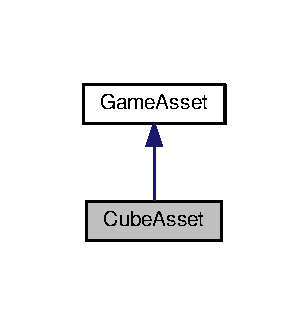
\includegraphics[width=148pt]{class_cube_asset__inherit__graph}
\end{center}
\end{figure}


Collaboration diagram for Cube\+Asset\+:
\nopagebreak
\begin{figure}[H]
\begin{center}
\leavevmode
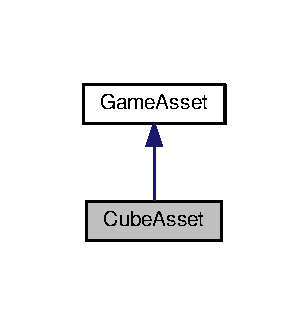
\includegraphics[width=148pt]{class_cube_asset__coll__graph}
\end{center}
\end{figure}
\subsection*{Public Member Functions}
\begin{DoxyCompactItemize}
\item 
\hyperlink{class_cube_asset_a615ed01cd3abb99e9fe55087a8a4ef0a}{Cube\+Asset} (int x, int y, int z)
\item 
\hyperlink{class_cube_asset_ab3ab9a5da82cbf8537a28652410093b1}{$\sim$\+Cube\+Asset} ()
\item 
virtual void \hyperlink{class_cube_asset_a1af568486056e254ffcf98fd99947bfe}{Draw} (G\+Luint)
\end{DoxyCompactItemize}
\subsection*{Private Attributes}
\begin{DoxyCompactItemize}
\item 
G\+Luint \hyperlink{class_cube_asset_ac66c2ec869f392515dad4ebda1fe4792}{element\+\_\+buffer\+\_\+length}
\item 
G\+Luint \hyperlink{class_cube_asset_a31bd098f60e2c24988316a9cc9335987}{vertex\+\_\+buffer\+\_\+token}
\item 
G\+Luint \hyperlink{class_cube_asset_a4fae699256e7c5633a8174a93ca8a0ec}{element\+\_\+buffer\+\_\+token}
\end{DoxyCompactItemize}


\subsection{Detailed Description}
Cube Asset Class -\/ Resonsible for storing structure of Cube class and drawing. 

Definition at line 15 of file Cube\+Asset.\+h.



\subsection{Constructor \& Destructor Documentation}
\hypertarget{class_cube_asset_a615ed01cd3abb99e9fe55087a8a4ef0a}{}\index{Cube\+Asset@{Cube\+Asset}!Cube\+Asset@{Cube\+Asset}}
\index{Cube\+Asset@{Cube\+Asset}!Cube\+Asset@{Cube\+Asset}}
\subsubsection[{Cube\+Asset(int x, int y, int z)}]{\setlength{\rightskip}{0pt plus 5cm}Cube\+Asset\+::\+Cube\+Asset (
\begin{DoxyParamCaption}
\item[{int}]{x, }
\item[{int}]{y, }
\item[{int}]{z}
\end{DoxyParamCaption}
)}\label{class_cube_asset_a615ed01cd3abb99e9fe55087a8a4ef0a}
Constructor -\/ Intialise vertices of cube x,y,z positions designed to modify positions of the cube(s) 

Definition at line 5 of file Cube\+Asset.\+cc.

\hypertarget{class_cube_asset_ab3ab9a5da82cbf8537a28652410093b1}{}\index{Cube\+Asset@{Cube\+Asset}!````~Cube\+Asset@{$\sim$\+Cube\+Asset}}
\index{````~Cube\+Asset@{$\sim$\+Cube\+Asset}!Cube\+Asset@{Cube\+Asset}}
\subsubsection[{$\sim$\+Cube\+Asset()}]{\setlength{\rightskip}{0pt plus 5cm}Cube\+Asset\+::$\sim$\+Cube\+Asset (
\begin{DoxyParamCaption}
{}
\end{DoxyParamCaption}
)}\label{class_cube_asset_ab3ab9a5da82cbf8537a28652410093b1}


Definition at line 61 of file Cube\+Asset.\+cc.



\subsection{Member Function Documentation}
\hypertarget{class_cube_asset_a1af568486056e254ffcf98fd99947bfe}{}\index{Cube\+Asset@{Cube\+Asset}!Draw@{Draw}}
\index{Draw@{Draw}!Cube\+Asset@{Cube\+Asset}}
\subsubsection[{Draw(\+G\+Luint)}]{\setlength{\rightskip}{0pt plus 5cm}void Cube\+Asset\+::\+Draw (
\begin{DoxyParamCaption}
\item[{G\+Luint}]{program\+\_\+token}
\end{DoxyParamCaption}
)\hspace{0.3cm}{\ttfamily [virtual]}}\label{class_cube_asset_a1af568486056e254ffcf98fd99947bfe}


Implements \hyperlink{class_game_asset_a961aa51ca0a9961fc584c0b5d5431300}{Game\+Asset}.



Definition at line 79 of file Cube\+Asset.\+cc.



\subsection{Member Data Documentation}
\hypertarget{class_cube_asset_ac66c2ec869f392515dad4ebda1fe4792}{}\index{Cube\+Asset@{Cube\+Asset}!element\+\_\+buffer\+\_\+length@{element\+\_\+buffer\+\_\+length}}
\index{element\+\_\+buffer\+\_\+length@{element\+\_\+buffer\+\_\+length}!Cube\+Asset@{Cube\+Asset}}
\subsubsection[{element\+\_\+buffer\+\_\+length}]{\setlength{\rightskip}{0pt plus 5cm}G\+Luint Cube\+Asset\+::element\+\_\+buffer\+\_\+length\hspace{0.3cm}{\ttfamily [private]}}\label{class_cube_asset_ac66c2ec869f392515dad4ebda1fe4792}
Resonsible for drawing and transferring information about Cube 

Definition at line 22 of file Cube\+Asset.\+h.

\hypertarget{class_cube_asset_a4fae699256e7c5633a8174a93ca8a0ec}{}\index{Cube\+Asset@{Cube\+Asset}!element\+\_\+buffer\+\_\+token@{element\+\_\+buffer\+\_\+token}}
\index{element\+\_\+buffer\+\_\+token@{element\+\_\+buffer\+\_\+token}!Cube\+Asset@{Cube\+Asset}}
\subsubsection[{element\+\_\+buffer\+\_\+token}]{\setlength{\rightskip}{0pt plus 5cm}G\+Luint Cube\+Asset\+::element\+\_\+buffer\+\_\+token\hspace{0.3cm}{\ttfamily [private]}}\label{class_cube_asset_a4fae699256e7c5633a8174a93ca8a0ec}
Three numbers (or each row) create a triangle. 

Definition at line 23 of file Cube\+Asset.\+h.

\hypertarget{class_cube_asset_a31bd098f60e2c24988316a9cc9335987}{}\index{Cube\+Asset@{Cube\+Asset}!vertex\+\_\+buffer\+\_\+token@{vertex\+\_\+buffer\+\_\+token}}
\index{vertex\+\_\+buffer\+\_\+token@{vertex\+\_\+buffer\+\_\+token}!Cube\+Asset@{Cube\+Asset}}
\subsubsection[{vertex\+\_\+buffer\+\_\+token}]{\setlength{\rightskip}{0pt plus 5cm}G\+Luint Cube\+Asset\+::vertex\+\_\+buffer\+\_\+token\hspace{0.3cm}{\ttfamily [private]}}\label{class_cube_asset_a31bd098f60e2c24988316a9cc9335987}
Store formed triangles which comprise cube

Each row defines a single vertex (or edge) of the cube in 3d space (x,y\&z positions). 

Definition at line 23 of file Cube\+Asset.\+h.



The documentation for this class was generated from the following files\+:\begin{DoxyCompactItemize}
\item 
src/\hyperlink{_cube_asset_8h}{Cube\+Asset.\+h}\item 
src/\hyperlink{_cube_asset_8cc}{Cube\+Asset.\+cc}\end{DoxyCompactItemize}

\hypertarget{class_game_asset}{}\section{Game\+Asset Class Reference}
\label{class_game_asset}\index{Game\+Asset@{Game\+Asset}}


{\ttfamily \#include $<$Game\+Asset.\+h$>$}



Inheritance diagram for Game\+Asset\+:\nopagebreak
\begin{figure}[H]
\begin{center}
\leavevmode
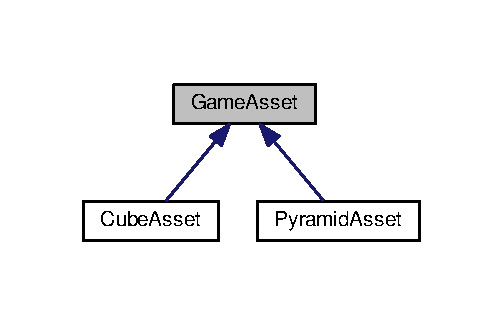
\includegraphics[width=242pt]{class_game_asset__inherit__graph}
\end{center}
\end{figure}
\subsection*{Public Member Functions}
\begin{DoxyCompactItemize}
\item 
virtual void \hyperlink{class_game_asset_a961aa51ca0a9961fc584c0b5d5431300}{Draw} (G\+Luint)=0
\end{DoxyCompactItemize}


\subsection{Detailed Description}
Abstract class 

Definition at line 11 of file Game\+Asset.\+h.



\subsection{Member Function Documentation}
\hypertarget{class_game_asset_a961aa51ca0a9961fc584c0b5d5431300}{}\index{Game\+Asset@{Game\+Asset}!Draw@{Draw}}
\index{Draw@{Draw}!Game\+Asset@{Game\+Asset}}
\subsubsection[{Draw(\+G\+Luint)=0}]{\setlength{\rightskip}{0pt plus 5cm}virtual void Game\+Asset\+::\+Draw (
\begin{DoxyParamCaption}
\item[{G\+Luint}]{}
\end{DoxyParamCaption}
)\hspace{0.3cm}{\ttfamily [pure virtual]}}\label{class_game_asset_a961aa51ca0a9961fc584c0b5d5431300}


Implemented in \hyperlink{class_cube_asset_a1af568486056e254ffcf98fd99947bfe}{Cube\+Asset}, and \hyperlink{class_pyramid_asset_aaea45da4956d79ec9ab96e9d0ccef3fe}{Pyramid\+Asset}.



The documentation for this class was generated from the following file\+:\begin{DoxyCompactItemize}
\item 
src/\hyperlink{_game_asset_8h}{Game\+Asset.\+h}\end{DoxyCompactItemize}

\hypertarget{class_game_asset_manager}{}\section{Game\+Asset\+Manager Class Reference}
\label{class_game_asset_manager}\index{Game\+Asset\+Manager@{Game\+Asset\+Manager}}


{\ttfamily \#include $<$Game\+Asset\+Manager.\+h$>$}



Collaboration diagram for Game\+Asset\+Manager\+:\nopagebreak
\begin{figure}[H]
\begin{center}
\leavevmode
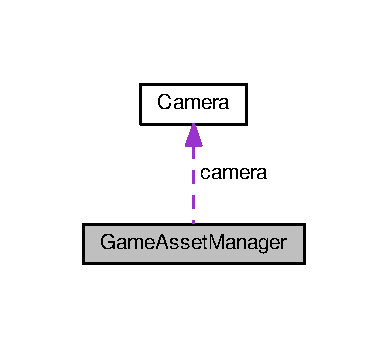
\includegraphics[width=186pt]{class_game_asset_manager__coll__graph}
\end{center}
\end{figure}
\subsection*{Public Member Functions}
\begin{DoxyCompactItemize}
\item 
\hyperlink{class_game_asset_manager_aaa0d58e276cc10ad91a7457085598a71}{Game\+Asset\+Manager} (\hyperlink{common_8h_add86e7c88dd109abea3f708b422f31f0}{Application\+Mode})
\item 
virtual \hyperlink{class_game_asset_manager_a1270bd61ecbcca563f079803e40c9b77}{$\sim$\+Game\+Asset\+Manager} ()
\item 
\hyperlink{class_game_asset_manager_a2c9adcb72faa154c87eadc9bafe5269d}{Game\+Asset\+Manager} (\hyperlink{class_game_asset_manager}{Game\+Asset\+Manager} const \&)
\item 
\hyperlink{class_game_asset_manager_a44f6e2fd6b8ff1dd64e5697f1be7386d}{Game\+Asset\+Manager} (\hyperlink{class_game_asset_manager}{Game\+Asset\+Manager} const \&\&)
\item 
void \hyperlink{class_game_asset_manager_ac72678a4ad5378c685aa6bae84a4e712}{operator=} (\hyperlink{class_game_asset_manager}{Game\+Asset\+Manager} const \&)
\item 
void \hyperlink{class_game_asset_manager_ad3de8ff00d55ba04728b1de8213b2349}{Add\+Asset} (std\+::shared\+\_\+ptr$<$ \hyperlink{class_game_asset}{Game\+Asset} $>$)
\item 
void \hyperlink{class_game_asset_manager_a32837132bd70a9a9ed537323c2d3d886}{Draw} ()
\item 
void \hyperlink{class_game_asset_manager_a2a2eeb7778b2955694cf2dd68f9daefb}{Update\+Camera\+Position} (\hyperlink{common_8h_a080a822f0093973313bd644e517a5090}{Input}, int mouse\+X, int mouse\+Y)
\end{DoxyCompactItemize}
\subsection*{Private Member Functions}
\begin{DoxyCompactItemize}
\item 
G\+Luint \hyperlink{class_game_asset_manager_abec45b44a8b35ad2d7d817ba10e0dd8d}{Create\+G\+L\+Program} (std\+::string \&, std\+::string \&)
\item 
G\+Luint \hyperlink{class_game_asset_manager_a1a1e5c07f941e8d3fda40d9442ac7037}{Create\+G\+L\+E\+S\+Shader} (G\+Lenum, std\+::string \&)
\item 
std\+::pair$<$ G\+Lchar $\ast$, G\+Lint $>$ \hyperlink{class_game_asset_manager_a23b124a213308a68a882727127601c97}{Read\+Shader} (std\+::string \&)
\end{DoxyCompactItemize}
\subsection*{Private Attributes}
\begin{DoxyCompactItemize}
\item 
std\+::vector$<$ std\+::shared\+\_\+ptr$<$ \hyperlink{class_game_asset}{Game\+Asset} $>$ $>$ \hyperlink{class_game_asset_manager_a671cddd92f1de4186c582fe0c4297b7d}{draw\+\_\+list}
\item 
G\+Luint \hyperlink{class_game_asset_manager_ad7bab17862e06ca692289f934b40548b}{program\+\_\+token}
\item 
\hyperlink{class_camera}{Camera} \hyperlink{class_game_asset_manager_af408912d75b4d97d29babc8850ecb8ae}{camera}
\item 
G\+Luint \hyperlink{class_game_asset_manager_a5e737710573e276ca53c683bc6731a51}{translate\+Matrix\+\_\+link}
\item 
G\+Luint \hyperlink{class_game_asset_manager_a71322a65c085d1d296e87aaddc4aea15}{view\+Matrix\+\_\+link}
\item 
G\+Luint \hyperlink{class_game_asset_manager_aa98eb0fb89a0a39e29be33294b322855}{projection\+Matrix\+\_\+link}
\item 
glm\+::mat4 \hyperlink{class_game_asset_manager_a1f0530749ec3ca5ee7925b2b70e8a8c2}{translate\+Matrix}
\item 
glm\+::mat4 \hyperlink{class_game_asset_manager_a4e702908c5d7d66e40c676d2c4f7930c}{view\+Matrix}
\item 
glm\+::mat4 \hyperlink{class_game_asset_manager_a2bc76e9ac72dcf9490436a59dc3bc752}{projection\+Matrix}
\item 
G\+Luint \hyperlink{class_game_asset_manager_a011295db68f0413a94700c5aa2778c45}{camera\+Position\+X}
\item 
G\+Luint \hyperlink{class_game_asset_manager_a076d00cef5f59a5038e168a0cc80420d}{camera\+Position\+Z}
\end{DoxyCompactItemize}


\subsection{Detailed Description}
\hyperlink{class_game_asset_manager}{Game\+Asset\+Manager} is a container for Game\+Assets. It also provides utility functions to to create a simple Open\+G\+L program that can be used to draw a simple \hyperlink{class_game_asset}{Game\+Asset}. 

Definition at line 24 of file Game\+Asset\+Manager.\+h.



\subsection{Constructor \& Destructor Documentation}
\hypertarget{class_game_asset_manager_aaa0d58e276cc10ad91a7457085598a71}{}\index{Game\+Asset\+Manager@{Game\+Asset\+Manager}!Game\+Asset\+Manager@{Game\+Asset\+Manager}}
\index{Game\+Asset\+Manager@{Game\+Asset\+Manager}!Game\+Asset\+Manager@{Game\+Asset\+Manager}}
\subsubsection[{Game\+Asset\+Manager(\+Application\+Mode)}]{\setlength{\rightskip}{0pt plus 5cm}Game\+Asset\+Manager\+::\+Game\+Asset\+Manager (
\begin{DoxyParamCaption}
\item[{{\bf Application\+Mode}}]{mode}
\end{DoxyParamCaption}
)\hspace{0.3cm}{\ttfamily [explicit]}}\label{class_game_asset_manager_aaa0d58e276cc10ad91a7457085598a71}
Creates a \hyperlink{class_game_asset_manager}{Game\+Asset\+Manager} to load the correct shaders based on the Application\+Mode. 

Definition at line 8 of file Game\+Asset\+Manager.\+cc.



Here is the call graph for this function\+:\nopagebreak
\begin{figure}[H]
\begin{center}
\leavevmode
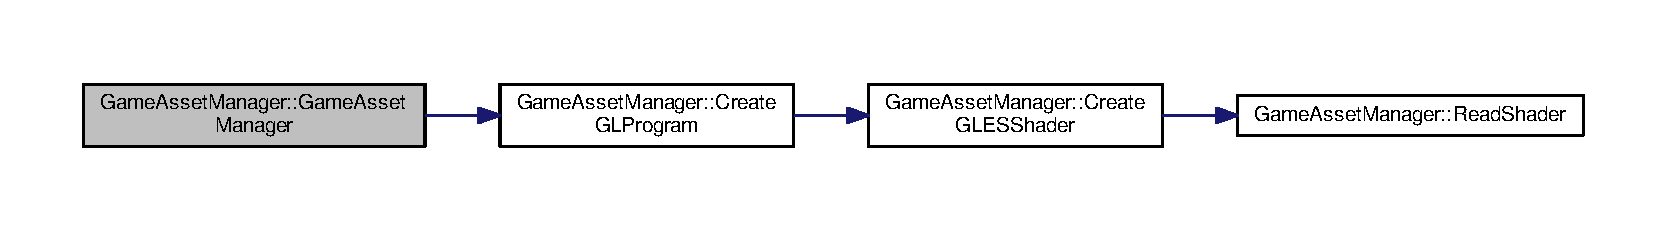
\includegraphics[width=350pt]{class_game_asset_manager_aaa0d58e276cc10ad91a7457085598a71_cgraph}
\end{center}
\end{figure}


\hypertarget{class_game_asset_manager_a1270bd61ecbcca563f079803e40c9b77}{}\index{Game\+Asset\+Manager@{Game\+Asset\+Manager}!````~Game\+Asset\+Manager@{$\sim$\+Game\+Asset\+Manager}}
\index{````~Game\+Asset\+Manager@{$\sim$\+Game\+Asset\+Manager}!Game\+Asset\+Manager@{Game\+Asset\+Manager}}
\subsubsection[{$\sim$\+Game\+Asset\+Manager()}]{\setlength{\rightskip}{0pt plus 5cm}Game\+Asset\+Manager\+::$\sim$\+Game\+Asset\+Manager (
\begin{DoxyParamCaption}
{}
\end{DoxyParamCaption}
)\hspace{0.3cm}{\ttfamily [virtual]}}\label{class_game_asset_manager_a1270bd61ecbcca563f079803e40c9b77}
Deletes a \hyperlink{class_game_asset_manager}{Game\+Asset\+Manager}, in particular it will clean up any modifications to the Open\+G\+L state. 

Definition at line 45 of file Game\+Asset\+Manager.\+cc.

\hypertarget{class_game_asset_manager_a2c9adcb72faa154c87eadc9bafe5269d}{}\index{Game\+Asset\+Manager@{Game\+Asset\+Manager}!Game\+Asset\+Manager@{Game\+Asset\+Manager}}
\index{Game\+Asset\+Manager@{Game\+Asset\+Manager}!Game\+Asset\+Manager@{Game\+Asset\+Manager}}
\subsubsection[{Game\+Asset\+Manager(\+Game\+Asset\+Manager const \&)}]{\setlength{\rightskip}{0pt plus 5cm}Game\+Asset\+Manager\+::\+Game\+Asset\+Manager (
\begin{DoxyParamCaption}
\item[{{\bf Game\+Asset\+Manager} const \&}]{the\+\_\+manager}
\end{DoxyParamCaption}
)}\label{class_game_asset_manager_a2c9adcb72faa154c87eadc9bafe5269d}
Unimplemented copy constructor -- this means that the \hyperlink{class_game_asset_manager}{Game\+Asset\+Manager} may not work as you\textquotesingle{}d expect when being copied. 

Definition at line 53 of file Game\+Asset\+Manager.\+cc.

\hypertarget{class_game_asset_manager_a44f6e2fd6b8ff1dd64e5697f1be7386d}{}\index{Game\+Asset\+Manager@{Game\+Asset\+Manager}!Game\+Asset\+Manager@{Game\+Asset\+Manager}}
\index{Game\+Asset\+Manager@{Game\+Asset\+Manager}!Game\+Asset\+Manager@{Game\+Asset\+Manager}}
\subsubsection[{Game\+Asset\+Manager(\+Game\+Asset\+Manager const \&\&)}]{\setlength{\rightskip}{0pt plus 5cm}Game\+Asset\+Manager\+::\+Game\+Asset\+Manager (
\begin{DoxyParamCaption}
\item[{{\bf Game\+Asset\+Manager} const \&\&}]{the\+\_\+manager}
\end{DoxyParamCaption}
)}\label{class_game_asset_manager_a44f6e2fd6b8ff1dd64e5697f1be7386d}
Unimplemented move constructor -- this unimplemented method violates the C++11 move semantics for \hyperlink{class_game_asset_manager}{Game\+Asset\+Manager}. 

Definition at line 61 of file Game\+Asset\+Manager.\+cc.



\subsection{Member Function Documentation}
\hypertarget{class_game_asset_manager_ad3de8ff00d55ba04728b1de8213b2349}{}\index{Game\+Asset\+Manager@{Game\+Asset\+Manager}!Add\+Asset@{Add\+Asset}}
\index{Add\+Asset@{Add\+Asset}!Game\+Asset\+Manager@{Game\+Asset\+Manager}}
\subsubsection[{Add\+Asset(std\+::shared\+\_\+ptr$<$ Game\+Asset $>$)}]{\setlength{\rightskip}{0pt plus 5cm}void Game\+Asset\+Manager\+::\+Add\+Asset (
\begin{DoxyParamCaption}
\item[{std\+::shared\+\_\+ptr$<$ {\bf Game\+Asset} $>$}]{the\+\_\+asset}
\end{DoxyParamCaption}
)}\label{class_game_asset_manager_ad3de8ff00d55ba04728b1de8213b2349}
Adds a \hyperlink{class_game_asset}{Game\+Asset} to the scene graph. 

Definition at line 76 of file Game\+Asset\+Manager.\+cc.

\hypertarget{class_game_asset_manager_a1a1e5c07f941e8d3fda40d9442ac7037}{}\index{Game\+Asset\+Manager@{Game\+Asset\+Manager}!Create\+G\+L\+E\+S\+Shader@{Create\+G\+L\+E\+S\+Shader}}
\index{Create\+G\+L\+E\+S\+Shader@{Create\+G\+L\+E\+S\+Shader}!Game\+Asset\+Manager@{Game\+Asset\+Manager}}
\subsubsection[{Create\+G\+L\+E\+S\+Shader(\+G\+Lenum, std\+::string \&)}]{\setlength{\rightskip}{0pt plus 5cm}G\+Luint Game\+Asset\+Manager\+::\+Create\+G\+L\+E\+S\+Shader (
\begin{DoxyParamCaption}
\item[{G\+Lenum}]{type, }
\item[{std\+::string \&}]{shader}
\end{DoxyParamCaption}
)\hspace{0.3cm}{\ttfamily [private]}}\label{class_game_asset_manager_a1a1e5c07f941e8d3fda40d9442ac7037}
When given a type of shader to construct and the contents of a shader, \hyperlink{class_game_asset_manager_a1a1e5c07f941e8d3fda40d9442ac7037}{Game\+Asset\+Manager\+::\+Create\+G\+L\+E\+S\+Shader} will create the shader or exit with error -\/1.

\begin{DoxyReturn}{Returns}
the G\+L \char`\"{}token\char`\"{} for the requested shader. 
\end{DoxyReturn}


Definition at line 132 of file Game\+Asset\+Manager.\+cc.



Here is the call graph for this function\+:\nopagebreak
\begin{figure}[H]
\begin{center}
\leavevmode
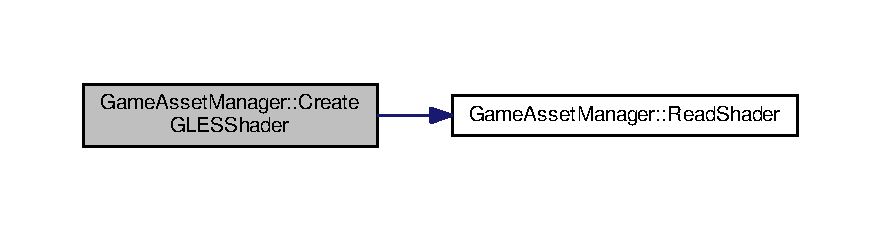
\includegraphics[width=350pt]{class_game_asset_manager_a1a1e5c07f941e8d3fda40d9442ac7037_cgraph}
\end{center}
\end{figure}


\hypertarget{class_game_asset_manager_abec45b44a8b35ad2d7d817ba10e0dd8d}{}\index{Game\+Asset\+Manager@{Game\+Asset\+Manager}!Create\+G\+L\+Program@{Create\+G\+L\+Program}}
\index{Create\+G\+L\+Program@{Create\+G\+L\+Program}!Game\+Asset\+Manager@{Game\+Asset\+Manager}}
\subsubsection[{Create\+G\+L\+Program(std\+::string \&, std\+::string \&)}]{\setlength{\rightskip}{0pt plus 5cm}G\+Luint Game\+Asset\+Manager\+::\+Create\+G\+L\+Program (
\begin{DoxyParamCaption}
\item[{std\+::string \&}]{vertex\+\_\+shader, }
\item[{std\+::string \&}]{fragment\+\_\+shader}
\end{DoxyParamCaption}
)\hspace{0.3cm}{\ttfamily [private]}}\label{class_game_asset_manager_abec45b44a8b35ad2d7d817ba10e0dd8d}
When given the contents of a vertex shader and fragment shader \hyperlink{class_game_asset_manager_abec45b44a8b35ad2d7d817ba10e0dd8d}{Game\+Asset\+Manager\+::\+Create\+G\+L\+Program} will compile and link them. This implementation will exit with -\/1 error if an error is detected.

\begin{DoxyReturn}{Returns}
the G\+L \char`\"{}token\char`\"{} referring to the gl program. 
\end{DoxyReturn}


Definition at line 102 of file Game\+Asset\+Manager.\+cc.



Here is the call graph for this function\+:\nopagebreak
\begin{figure}[H]
\begin{center}
\leavevmode
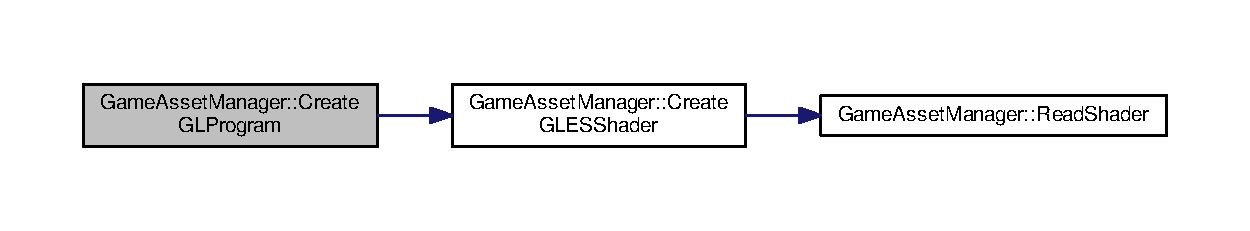
\includegraphics[width=350pt]{class_game_asset_manager_abec45b44a8b35ad2d7d817ba10e0dd8d_cgraph}
\end{center}
\end{figure}


\hypertarget{class_game_asset_manager_a32837132bd70a9a9ed537323c2d3d886}{}\index{Game\+Asset\+Manager@{Game\+Asset\+Manager}!Draw@{Draw}}
\index{Draw@{Draw}!Game\+Asset\+Manager@{Game\+Asset\+Manager}}
\subsubsection[{Draw()}]{\setlength{\rightskip}{0pt plus 5cm}void Game\+Asset\+Manager\+::\+Draw (
\begin{DoxyParamCaption}
{}
\end{DoxyParamCaption}
)}\label{class_game_asset_manager_a32837132bd70a9a9ed537323c2d3d886}
Draws each \hyperlink{class_game_asset}{Game\+Asset} in the scene graph. 

Definition at line 83 of file Game\+Asset\+Manager.\+cc.

\hypertarget{class_game_asset_manager_ac72678a4ad5378c685aa6bae84a4e712}{}\index{Game\+Asset\+Manager@{Game\+Asset\+Manager}!operator=@{operator=}}
\index{operator=@{operator=}!Game\+Asset\+Manager@{Game\+Asset\+Manager}}
\subsubsection[{operator=(\+Game\+Asset\+Manager const \&)}]{\setlength{\rightskip}{0pt plus 5cm}void Game\+Asset\+Manager\+::operator= (
\begin{DoxyParamCaption}
\item[{{\bf Game\+Asset\+Manager} const \&}]{the\+\_\+manager}
\end{DoxyParamCaption}
)}\label{class_game_asset_manager_ac72678a4ad5378c685aa6bae84a4e712}
Unimplemented assisgnment operator -- violates the expected semantics for assignment in C++11. 

Definition at line 69 of file Game\+Asset\+Manager.\+cc.

\hypertarget{class_game_asset_manager_a23b124a213308a68a882727127601c97}{}\index{Game\+Asset\+Manager@{Game\+Asset\+Manager}!Read\+Shader@{Read\+Shader}}
\index{Read\+Shader@{Read\+Shader}!Game\+Asset\+Manager@{Game\+Asset\+Manager}}
\subsubsection[{Read\+Shader(std\+::string \&)}]{\setlength{\rightskip}{0pt plus 5cm}std\+::pair$<$ G\+Lchar $\ast$, G\+Lint $>$ Game\+Asset\+Manager\+::\+Read\+Shader (
\begin{DoxyParamCaption}
\item[{std\+::string \&}]{shader}
\end{DoxyParamCaption}
)\hspace{0.3cm}{\ttfamily [private]}}\label{class_game_asset_manager_a23b124a213308a68a882727127601c97}
Read\+Shader reads the contents of a file and packs it into a null termintated G\+Lchar $\ast$ which is suitable for sending to Open\+G\+L.

\begin{DoxyReturn}{Returns}
a pair consisting of the shader file contents and a holder for the Open\+G\+L \char`\"{}token\char`\"{}. 
\end{DoxyReturn}


Definition at line 173 of file Game\+Asset\+Manager.\+cc.

\hypertarget{class_game_asset_manager_a2a2eeb7778b2955694cf2dd68f9daefb}{}\index{Game\+Asset\+Manager@{Game\+Asset\+Manager}!Update\+Camera\+Position@{Update\+Camera\+Position}}
\index{Update\+Camera\+Position@{Update\+Camera\+Position}!Game\+Asset\+Manager@{Game\+Asset\+Manager}}
\subsubsection[{Update\+Camera\+Position(\+Input, int mouse\+X, int mouse\+Y)}]{\setlength{\rightskip}{0pt plus 5cm}void Game\+Asset\+Manager\+::\+Update\+Camera\+Position (
\begin{DoxyParamCaption}
\item[{{\bf Input}}]{input\+\_\+\+Direction, }
\item[{int}]{mouse\+X, }
\item[{int}]{mouse\+Y}
\end{DoxyParamCaption}
)}\label{class_game_asset_manager_a2a2eeb7778b2955694cf2dd68f9daefb}


Definition at line 34 of file Game\+Asset\+Manager.\+cc.



Here is the call graph for this function\+:\nopagebreak
\begin{figure}[H]
\begin{center}
\leavevmode
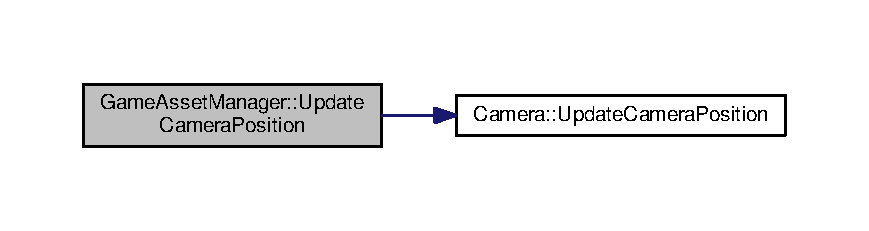
\includegraphics[width=350pt]{class_game_asset_manager_a2a2eeb7778b2955694cf2dd68f9daefb_cgraph}
\end{center}
\end{figure}




\subsection{Member Data Documentation}
\hypertarget{class_game_asset_manager_af408912d75b4d97d29babc8850ecb8ae}{}\index{Game\+Asset\+Manager@{Game\+Asset\+Manager}!camera@{camera}}
\index{camera@{camera}!Game\+Asset\+Manager@{Game\+Asset\+Manager}}
\subsubsection[{camera}]{\setlength{\rightskip}{0pt plus 5cm}{\bf Camera} Game\+Asset\+Manager\+::camera\hspace{0.3cm}{\ttfamily [private]}}\label{class_game_asset_manager_af408912d75b4d97d29babc8850ecb8ae}


Definition at line 46 of file Game\+Asset\+Manager.\+h.

\hypertarget{class_game_asset_manager_a011295db68f0413a94700c5aa2778c45}{}\index{Game\+Asset\+Manager@{Game\+Asset\+Manager}!camera\+Position\+X@{camera\+Position\+X}}
\index{camera\+Position\+X@{camera\+Position\+X}!Game\+Asset\+Manager@{Game\+Asset\+Manager}}
\subsubsection[{camera\+Position\+X}]{\setlength{\rightskip}{0pt plus 5cm}G\+Luint Game\+Asset\+Manager\+::camera\+Position\+X\hspace{0.3cm}{\ttfamily [private]}}\label{class_game_asset_manager_a011295db68f0413a94700c5aa2778c45}


Definition at line 56 of file Game\+Asset\+Manager.\+h.

\hypertarget{class_game_asset_manager_a076d00cef5f59a5038e168a0cc80420d}{}\index{Game\+Asset\+Manager@{Game\+Asset\+Manager}!camera\+Position\+Z@{camera\+Position\+Z}}
\index{camera\+Position\+Z@{camera\+Position\+Z}!Game\+Asset\+Manager@{Game\+Asset\+Manager}}
\subsubsection[{camera\+Position\+Z}]{\setlength{\rightskip}{0pt plus 5cm}G\+Luint Game\+Asset\+Manager\+::camera\+Position\+Z\hspace{0.3cm}{\ttfamily [private]}}\label{class_game_asset_manager_a076d00cef5f59a5038e168a0cc80420d}


Definition at line 57 of file Game\+Asset\+Manager.\+h.

\hypertarget{class_game_asset_manager_a671cddd92f1de4186c582fe0c4297b7d}{}\index{Game\+Asset\+Manager@{Game\+Asset\+Manager}!draw\+\_\+list@{draw\+\_\+list}}
\index{draw\+\_\+list@{draw\+\_\+list}!Game\+Asset\+Manager@{Game\+Asset\+Manager}}
\subsubsection[{draw\+\_\+list}]{\setlength{\rightskip}{0pt plus 5cm}std\+::vector$<$std\+::shared\+\_\+ptr$<${\bf Game\+Asset}$>$ $>$ Game\+Asset\+Manager\+::draw\+\_\+list\hspace{0.3cm}{\ttfamily [private]}}\label{class_game_asset_manager_a671cddd92f1de4186c582fe0c4297b7d}


Definition at line 44 of file Game\+Asset\+Manager.\+h.

\hypertarget{class_game_asset_manager_ad7bab17862e06ca692289f934b40548b}{}\index{Game\+Asset\+Manager@{Game\+Asset\+Manager}!program\+\_\+token@{program\+\_\+token}}
\index{program\+\_\+token@{program\+\_\+token}!Game\+Asset\+Manager@{Game\+Asset\+Manager}}
\subsubsection[{program\+\_\+token}]{\setlength{\rightskip}{0pt plus 5cm}G\+Luint Game\+Asset\+Manager\+::program\+\_\+token\hspace{0.3cm}{\ttfamily [private]}}\label{class_game_asset_manager_ad7bab17862e06ca692289f934b40548b}


Definition at line 45 of file Game\+Asset\+Manager.\+h.

\hypertarget{class_game_asset_manager_a2bc76e9ac72dcf9490436a59dc3bc752}{}\index{Game\+Asset\+Manager@{Game\+Asset\+Manager}!projection\+Matrix@{projection\+Matrix}}
\index{projection\+Matrix@{projection\+Matrix}!Game\+Asset\+Manager@{Game\+Asset\+Manager}}
\subsubsection[{projection\+Matrix}]{\setlength{\rightskip}{0pt plus 5cm}glm\+::mat4 Game\+Asset\+Manager\+::projection\+Matrix\hspace{0.3cm}{\ttfamily [private]}}\label{class_game_asset_manager_a2bc76e9ac72dcf9490436a59dc3bc752}


Definition at line 54 of file Game\+Asset\+Manager.\+h.

\hypertarget{class_game_asset_manager_aa98eb0fb89a0a39e29be33294b322855}{}\index{Game\+Asset\+Manager@{Game\+Asset\+Manager}!projection\+Matrix\+\_\+link@{projection\+Matrix\+\_\+link}}
\index{projection\+Matrix\+\_\+link@{projection\+Matrix\+\_\+link}!Game\+Asset\+Manager@{Game\+Asset\+Manager}}
\subsubsection[{projection\+Matrix\+\_\+link}]{\setlength{\rightskip}{0pt plus 5cm}G\+Luint Game\+Asset\+Manager\+::projection\+Matrix\+\_\+link\hspace{0.3cm}{\ttfamily [private]}}\label{class_game_asset_manager_aa98eb0fb89a0a39e29be33294b322855}


Definition at line 50 of file Game\+Asset\+Manager.\+h.

\hypertarget{class_game_asset_manager_a1f0530749ec3ca5ee7925b2b70e8a8c2}{}\index{Game\+Asset\+Manager@{Game\+Asset\+Manager}!translate\+Matrix@{translate\+Matrix}}
\index{translate\+Matrix@{translate\+Matrix}!Game\+Asset\+Manager@{Game\+Asset\+Manager}}
\subsubsection[{translate\+Matrix}]{\setlength{\rightskip}{0pt plus 5cm}glm\+::mat4 Game\+Asset\+Manager\+::translate\+Matrix\hspace{0.3cm}{\ttfamily [private]}}\label{class_game_asset_manager_a1f0530749ec3ca5ee7925b2b70e8a8c2}


Definition at line 52 of file Game\+Asset\+Manager.\+h.

\hypertarget{class_game_asset_manager_a5e737710573e276ca53c683bc6731a51}{}\index{Game\+Asset\+Manager@{Game\+Asset\+Manager}!translate\+Matrix\+\_\+link@{translate\+Matrix\+\_\+link}}
\index{translate\+Matrix\+\_\+link@{translate\+Matrix\+\_\+link}!Game\+Asset\+Manager@{Game\+Asset\+Manager}}
\subsubsection[{translate\+Matrix\+\_\+link}]{\setlength{\rightskip}{0pt plus 5cm}G\+Luint Game\+Asset\+Manager\+::translate\+Matrix\+\_\+link\hspace{0.3cm}{\ttfamily [private]}}\label{class_game_asset_manager_a5e737710573e276ca53c683bc6731a51}


Definition at line 48 of file Game\+Asset\+Manager.\+h.

\hypertarget{class_game_asset_manager_a4e702908c5d7d66e40c676d2c4f7930c}{}\index{Game\+Asset\+Manager@{Game\+Asset\+Manager}!view\+Matrix@{view\+Matrix}}
\index{view\+Matrix@{view\+Matrix}!Game\+Asset\+Manager@{Game\+Asset\+Manager}}
\subsubsection[{view\+Matrix}]{\setlength{\rightskip}{0pt plus 5cm}glm\+::mat4 Game\+Asset\+Manager\+::view\+Matrix\hspace{0.3cm}{\ttfamily [private]}}\label{class_game_asset_manager_a4e702908c5d7d66e40c676d2c4f7930c}


Definition at line 53 of file Game\+Asset\+Manager.\+h.

\hypertarget{class_game_asset_manager_a71322a65c085d1d296e87aaddc4aea15}{}\index{Game\+Asset\+Manager@{Game\+Asset\+Manager}!view\+Matrix\+\_\+link@{view\+Matrix\+\_\+link}}
\index{view\+Matrix\+\_\+link@{view\+Matrix\+\_\+link}!Game\+Asset\+Manager@{Game\+Asset\+Manager}}
\subsubsection[{view\+Matrix\+\_\+link}]{\setlength{\rightskip}{0pt plus 5cm}G\+Luint Game\+Asset\+Manager\+::view\+Matrix\+\_\+link\hspace{0.3cm}{\ttfamily [private]}}\label{class_game_asset_manager_a71322a65c085d1d296e87aaddc4aea15}


Definition at line 49 of file Game\+Asset\+Manager.\+h.



The documentation for this class was generated from the following files\+:\begin{DoxyCompactItemize}
\item 
src/\hyperlink{_game_asset_manager_8h}{Game\+Asset\+Manager.\+h}\item 
src/\hyperlink{_game_asset_manager_8cc}{Game\+Asset\+Manager.\+cc}\end{DoxyCompactItemize}

\hypertarget{class_game_world}{}\section{Game\+World Class Reference}
\label{class_game_world}\index{Game\+World@{Game\+World}}


{\ttfamily \#include $<$Game\+World.\+h$>$}

\subsection*{Public Member Functions}
\begin{DoxyCompactItemize}
\item 
\hyperlink{class_game_world_a17a84e57a80600961088afc753036f89}{Game\+World} (\hyperlink{common_8h_add86e7c88dd109abea3f708b422f31f0}{Application\+Mode})
\item 
void \hyperlink{class_game_world_a275418607d8286979b276f165ad5876b}{Draw} ()
\item 
void \hyperlink{class_game_world_aa934714929b8b3bcf322f1ec4695d75b}{Update\+Camera\+Position} (\hyperlink{common_8h_a080a822f0093973313bd644e517a5090}{Input}, int mouse\+X, int mouse\+Y)
\end{DoxyCompactItemize}
\subsection*{Private Attributes}
\begin{DoxyCompactItemize}
\item 
std\+::shared\+\_\+ptr$<$ \hyperlink{class_game_asset_manager}{Game\+Asset\+Manager} $>$ \hyperlink{class_game_world_aec5c0bca4fb5a41e4aac2dce2871266d}{asset\+\_\+manager}
\end{DoxyCompactItemize}


\subsection{Detailed Description}
\hyperlink{class_game_world}{Game\+World} allows us to separate the management of the game world from the nuts and bolts of game loop initialisation. The \hyperlink{class_game_world}{Game\+World} currently has a very simplified scene graph consisiting of a single \hyperlink{class_game_asset_manager}{Game\+Asset\+Manager}. 

Definition at line 18 of file Game\+World.\+h.



\subsection{Constructor \& Destructor Documentation}
\hypertarget{class_game_world_a17a84e57a80600961088afc753036f89}{}\index{Game\+World@{Game\+World}!Game\+World@{Game\+World}}
\index{Game\+World@{Game\+World}!Game\+World@{Game\+World}}
\subsubsection[{Game\+World(\+Application\+Mode)}]{\setlength{\rightskip}{0pt plus 5cm}Game\+World\+::\+Game\+World (
\begin{DoxyParamCaption}
\item[{{\bf Application\+Mode}}]{mode}
\end{DoxyParamCaption}
)}\label{class_game_world_a17a84e57a80600961088afc753036f89}
We thread the Application\+Mode through the \hyperlink{class_game_world}{Game\+World} ss we want to read it in from the user. Threading the state through the various function calls is preferable (in this case) to having some kind of global state.

\hyperlink{class_game_world}{Game\+World} class -\/ responsible for holding information about the world and applying draw commands 3\+D Array to store block world configuration 

Definition at line 9 of file Game\+World.\+cc.



\subsection{Member Function Documentation}
\hypertarget{class_game_world_a275418607d8286979b276f165ad5876b}{}\index{Game\+World@{Game\+World}!Draw@{Draw}}
\index{Draw@{Draw}!Game\+World@{Game\+World}}
\subsubsection[{Draw()}]{\setlength{\rightskip}{0pt plus 5cm}void Game\+World\+::\+Draw (
\begin{DoxyParamCaption}
{}
\end{DoxyParamCaption}
)}\label{class_game_world_a275418607d8286979b276f165ad5876b}
Calling \hyperlink{class_game_world_a275418607d8286979b276f165ad5876b}{Draw()} will draw the entire world. 

Definition at line 66 of file Game\+World.\+cc.

\hypertarget{class_game_world_aa934714929b8b3bcf322f1ec4695d75b}{}\index{Game\+World@{Game\+World}!Update\+Camera\+Position@{Update\+Camera\+Position}}
\index{Update\+Camera\+Position@{Update\+Camera\+Position}!Game\+World@{Game\+World}}
\subsubsection[{Update\+Camera\+Position(\+Input, int mouse\+X, int mouse\+Y)}]{\setlength{\rightskip}{0pt plus 5cm}void Game\+World\+::\+Update\+Camera\+Position (
\begin{DoxyParamCaption}
\item[{{\bf Input}}]{input\+\_\+direction, }
\item[{int}]{mouse\+X, }
\item[{int}]{mouse\+Y}
\end{DoxyParamCaption}
)}\label{class_game_world_aa934714929b8b3bcf322f1ec4695d75b}


Definition at line 71 of file Game\+World.\+cc.



\subsection{Member Data Documentation}
\hypertarget{class_game_world_aec5c0bca4fb5a41e4aac2dce2871266d}{}\index{Game\+World@{Game\+World}!asset\+\_\+manager@{asset\+\_\+manager}}
\index{asset\+\_\+manager@{asset\+\_\+manager}!Game\+World@{Game\+World}}
\subsubsection[{asset\+\_\+manager}]{\setlength{\rightskip}{0pt plus 5cm}std\+::shared\+\_\+ptr$<${\bf Game\+Asset\+Manager}$>$ Game\+World\+::asset\+\_\+manager\hspace{0.3cm}{\ttfamily [private]}}\label{class_game_world_aec5c0bca4fb5a41e4aac2dce2871266d}


Definition at line 35 of file Game\+World.\+h.



The documentation for this class was generated from the following files\+:\begin{DoxyCompactItemize}
\item 
src/\hyperlink{_game_world_8h}{Game\+World.\+h}\item 
src/\hyperlink{_game_world_8cc}{Game\+World.\+cc}\end{DoxyCompactItemize}

\hypertarget{struct_s_d_l_window_deleter}{}\section{S\+D\+L\+Window\+Deleter Struct Reference}
\label{struct_s_d_l_window_deleter}\index{S\+D\+L\+Window\+Deleter@{S\+D\+L\+Window\+Deleter}}
\subsection*{Public Member Functions}
\begin{DoxyCompactItemize}
\item 
void \hyperlink{struct_s_d_l_window_deleter_a2aedcc99c3756ae090c38badabeb10b1}{operator()} (S\+D\+L\+\_\+\+Window $\ast$window)
\end{DoxyCompactItemize}


\subsection{Detailed Description}


Definition at line 33 of file main.\+cc.



\subsection{Member Function Documentation}
\hypertarget{struct_s_d_l_window_deleter_a2aedcc99c3756ae090c38badabeb10b1}{}\index{S\+D\+L\+Window\+Deleter@{S\+D\+L\+Window\+Deleter}!operator()@{operator()}}
\index{operator()@{operator()}!S\+D\+L\+Window\+Deleter@{S\+D\+L\+Window\+Deleter}}
\subsubsection[{operator()(\+S\+D\+L\+\_\+\+Window $\ast$window)}]{\setlength{\rightskip}{0pt plus 5cm}void S\+D\+L\+Window\+Deleter\+::operator() (
\begin{DoxyParamCaption}
\item[{S\+D\+L\+\_\+\+Window $\ast$}]{window}
\end{DoxyParamCaption}
)\hspace{0.3cm}{\ttfamily [inline]}}\label{struct_s_d_l_window_deleter_a2aedcc99c3756ae090c38badabeb10b1}


Definition at line 34 of file main.\+cc.



The documentation for this struct was generated from the following file\+:\begin{DoxyCompactItemize}
\item 
src/\hyperlink{main_8cc}{main.\+cc}\end{DoxyCompactItemize}

\chapter{File Documentation}
\hypertarget{common_8h}{}\section{src/common.h File Reference}
\label{common_8h}\index{src/common.\+h@{src/common.\+h}}
This graph shows which files directly or indirectly include this file\+:
\nopagebreak
\begin{figure}[H]
\begin{center}
\leavevmode
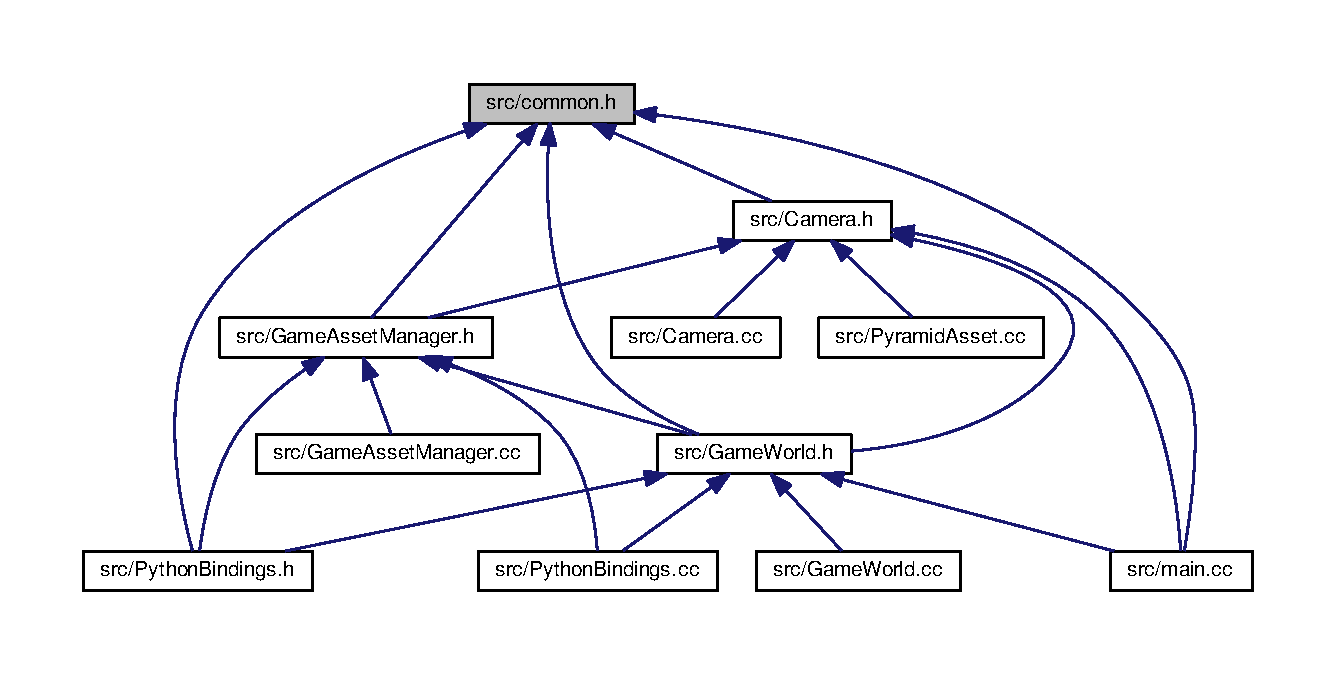
\includegraphics[width=350pt]{common_8h__dep__incl}
\end{center}
\end{figure}
\subsection*{Enumerations}
\begin{DoxyCompactItemize}
\item 
enum \hyperlink{common_8h_add86e7c88dd109abea3f708b422f31f0}{Application\+Mode} \{ \hyperlink{common_8h_add86e7c88dd109abea3f708b422f31f0a25f73324dc93d9024c0c75b4e6815335}{T\+R\+A\+N\+S\+F\+O\+R\+M}, 
\hyperlink{common_8h_add86e7c88dd109abea3f708b422f31f0a3dcfe0046eb5876e287dbf0914819b16}{R\+O\+T\+A\+T\+E}, 
\hyperlink{common_8h_add86e7c88dd109abea3f708b422f31f0a593be05a10070b4e7e0856e20590eaaf}{S\+C\+A\+L\+E}
 \}
\end{DoxyCompactItemize}


\subsection{Enumeration Type Documentation}
\hypertarget{common_8h_add86e7c88dd109abea3f708b422f31f0}{}\index{common.\+h@{common.\+h}!Application\+Mode@{Application\+Mode}}
\index{Application\+Mode@{Application\+Mode}!common.\+h@{common.\+h}}
\subsubsection[{Application\+Mode}]{\setlength{\rightskip}{0pt plus 5cm}enum {\bf Application\+Mode}}\label{common_8h_add86e7c88dd109abea3f708b422f31f0}
Application\+Mode denotes the global state of the application. There are three global states for this application\+:
\begin{DoxyEnumerate}
\item Transform -- load the correct shaders to do a transformation of a simple asset.
\item Rotate -- load the correct shader to rotate a simple asset.
\item Scale -- load the correct shader to scale a simple asset. 
\end{DoxyEnumerate}\begin{Desc}
\item[Enumerator]\par
\begin{description}
\index{T\+R\+A\+N\+S\+F\+O\+R\+M@{T\+R\+A\+N\+S\+F\+O\+R\+M}!common.\+h@{common.\+h}}\index{common.\+h@{common.\+h}!T\+R\+A\+N\+S\+F\+O\+R\+M@{T\+R\+A\+N\+S\+F\+O\+R\+M}}\item[{\em 
\hypertarget{common_8h_add86e7c88dd109abea3f708b422f31f0a25f73324dc93d9024c0c75b4e6815335}{}T\+R\+A\+N\+S\+F\+O\+R\+M\label{common_8h_add86e7c88dd109abea3f708b422f31f0a25f73324dc93d9024c0c75b4e6815335}
}]\index{R\+O\+T\+A\+T\+E@{R\+O\+T\+A\+T\+E}!common.\+h@{common.\+h}}\index{common.\+h@{common.\+h}!R\+O\+T\+A\+T\+E@{R\+O\+T\+A\+T\+E}}\item[{\em 
\hypertarget{common_8h_add86e7c88dd109abea3f708b422f31f0a3dcfe0046eb5876e287dbf0914819b16}{}R\+O\+T\+A\+T\+E\label{common_8h_add86e7c88dd109abea3f708b422f31f0a3dcfe0046eb5876e287dbf0914819b16}
}]\index{S\+C\+A\+L\+E@{S\+C\+A\+L\+E}!common.\+h@{common.\+h}}\index{common.\+h@{common.\+h}!S\+C\+A\+L\+E@{S\+C\+A\+L\+E}}\item[{\em 
\hypertarget{common_8h_add86e7c88dd109abea3f708b422f31f0a593be05a10070b4e7e0856e20590eaaf}{}S\+C\+A\+L\+E\label{common_8h_add86e7c88dd109abea3f708b422f31f0a593be05a10070b4e7e0856e20590eaaf}
}]\end{description}
\end{Desc}


Definition at line 12 of file common.\+h.


\hypertarget{_cube_asset_8cc}{}\section{src/\+Cube\+Asset.cc File Reference}
\label{_cube_asset_8cc}\index{src/\+Cube\+Asset.\+cc@{src/\+Cube\+Asset.\+cc}}
{\ttfamily \#include \char`\"{}Cube\+Asset.\+h\char`\"{}}\\*
Include dependency graph for Cube\+Asset.\+cc\+:\nopagebreak
\begin{figure}[H]
\begin{center}
\leavevmode
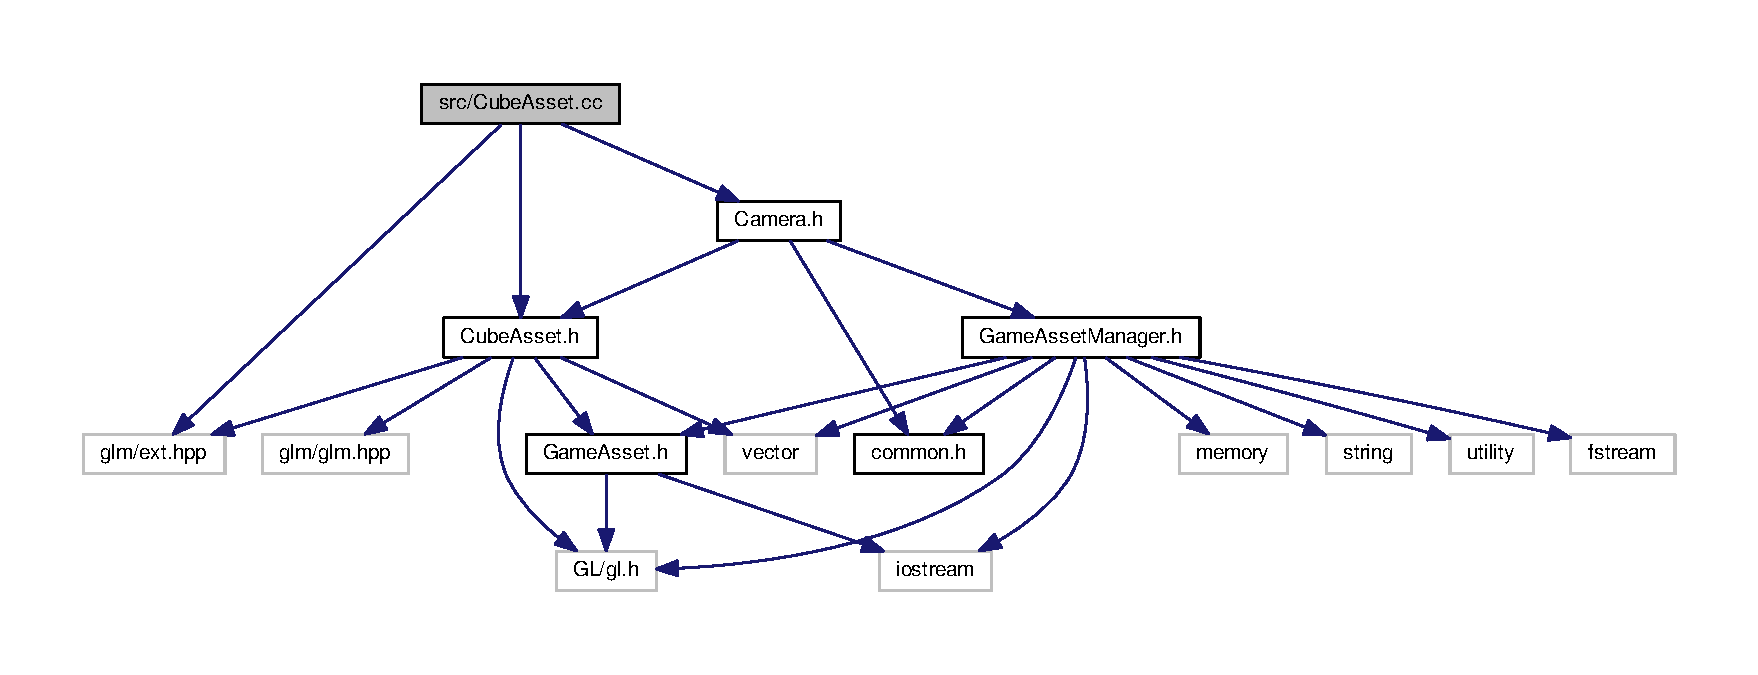
\includegraphics[width=350pt]{_cube_asset_8cc__incl}
\end{center}
\end{figure}
\subsection*{Macros}
\begin{DoxyCompactItemize}
\item 
\#define \hyperlink{_cube_asset_8cc_a75f201b0e53e68726854997957322b8d}{check\+G\+L\+Error}()
\end{DoxyCompactItemize}
\subsection*{Functions}
\begin{DoxyCompactItemize}
\item 
void \hyperlink{_cube_asset_8cc_abe4ebf09b25b6e092e65ce01e73987d7}{check\+Error} (std\+::string file, int line)
\end{DoxyCompactItemize}


\subsection{Macro Definition Documentation}
\hypertarget{_cube_asset_8cc_a75f201b0e53e68726854997957322b8d}{}\index{Cube\+Asset.\+cc@{Cube\+Asset.\+cc}!check\+G\+L\+Error@{check\+G\+L\+Error}}
\index{check\+G\+L\+Error@{check\+G\+L\+Error}!Cube\+Asset.\+cc@{Cube\+Asset.\+cc}}
\subsubsection[{check\+G\+L\+Error}]{\setlength{\rightskip}{0pt plus 5cm}\#define check\+G\+L\+Error(
\begin{DoxyParamCaption}
{}
\end{DoxyParamCaption}
)}\label{_cube_asset_8cc_a75f201b0e53e68726854997957322b8d}


Definition at line 104 of file Cube\+Asset.\+cc.



\subsection{Function Documentation}
\hypertarget{_cube_asset_8cc_abe4ebf09b25b6e092e65ce01e73987d7}{}\index{Cube\+Asset.\+cc@{Cube\+Asset.\+cc}!check\+Error@{check\+Error}}
\index{check\+Error@{check\+Error}!Cube\+Asset.\+cc@{Cube\+Asset.\+cc}}
\subsubsection[{check\+Error(std\+::string file, int line)}]{\setlength{\rightskip}{0pt plus 5cm}void check\+Error (
\begin{DoxyParamCaption}
\item[{std\+::string}]{file, }
\item[{int}]{line}
\end{DoxyParamCaption}
)}\label{_cube_asset_8cc_abe4ebf09b25b6e092e65ce01e73987d7}


Definition at line 107 of file Cube\+Asset.\+cc.


\hypertarget{_cube_asset_8h}{}\section{src/\+Cube\+Asset.h File Reference}
\label{_cube_asset_8h}\index{src/\+Cube\+Asset.\+h@{src/\+Cube\+Asset.\+h}}
{\ttfamily \#include $<$vector$>$}\\*
{\ttfamily \#include $<$G\+L/gl.\+h$>$}\\*
{\ttfamily \#include $<$glm/glm.\+hpp$>$}\\*
{\ttfamily \#include $<$glm/ext.\+hpp$>$}\\*
{\ttfamily \#include \char`\"{}Game\+Asset.\+h\char`\"{}}\\*
Include dependency graph for Cube\+Asset.\+h\+:\nopagebreak
\begin{figure}[H]
\begin{center}
\leavevmode
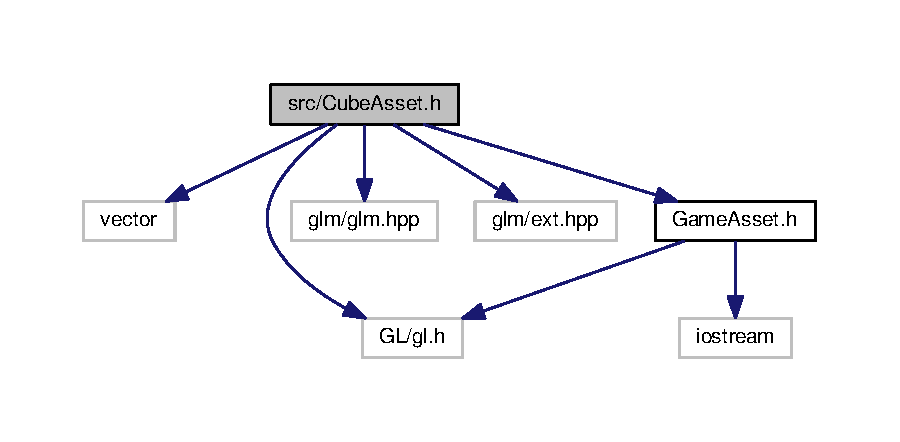
\includegraphics[width=350pt]{_cube_asset_8h__incl}
\end{center}
\end{figure}
This graph shows which files directly or indirectly include this file\+:\nopagebreak
\begin{figure}[H]
\begin{center}
\leavevmode
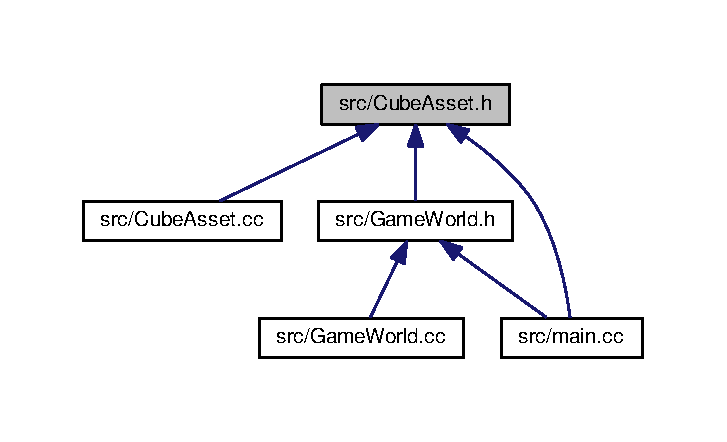
\includegraphics[width=350pt]{_cube_asset_8h__dep__incl}
\end{center}
\end{figure}
\subsection*{Classes}
\begin{DoxyCompactItemize}
\item 
class \hyperlink{class_cube_asset}{Cube\+Asset}
\end{DoxyCompactItemize}

\hypertarget{_game_asset_8h}{}\section{src/\+Game\+Asset.h File Reference}
\label{_game_asset_8h}\index{src/\+Game\+Asset.\+h@{src/\+Game\+Asset.\+h}}
{\ttfamily \#include $<$iostream$>$}\\*
{\ttfamily \#include $<$G\+L/gl.\+h$>$}\\*
Include dependency graph for Game\+Asset.\+h\+:\nopagebreak
\begin{figure}[H]
\begin{center}
\leavevmode
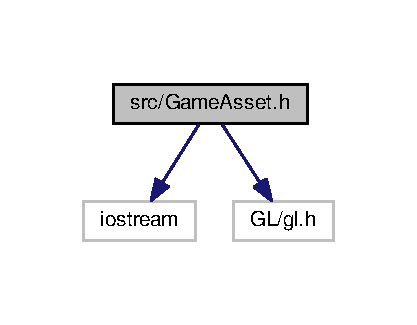
\includegraphics[width=200pt]{_game_asset_8h__incl}
\end{center}
\end{figure}
This graph shows which files directly or indirectly include this file\+:
\nopagebreak
\begin{figure}[H]
\begin{center}
\leavevmode
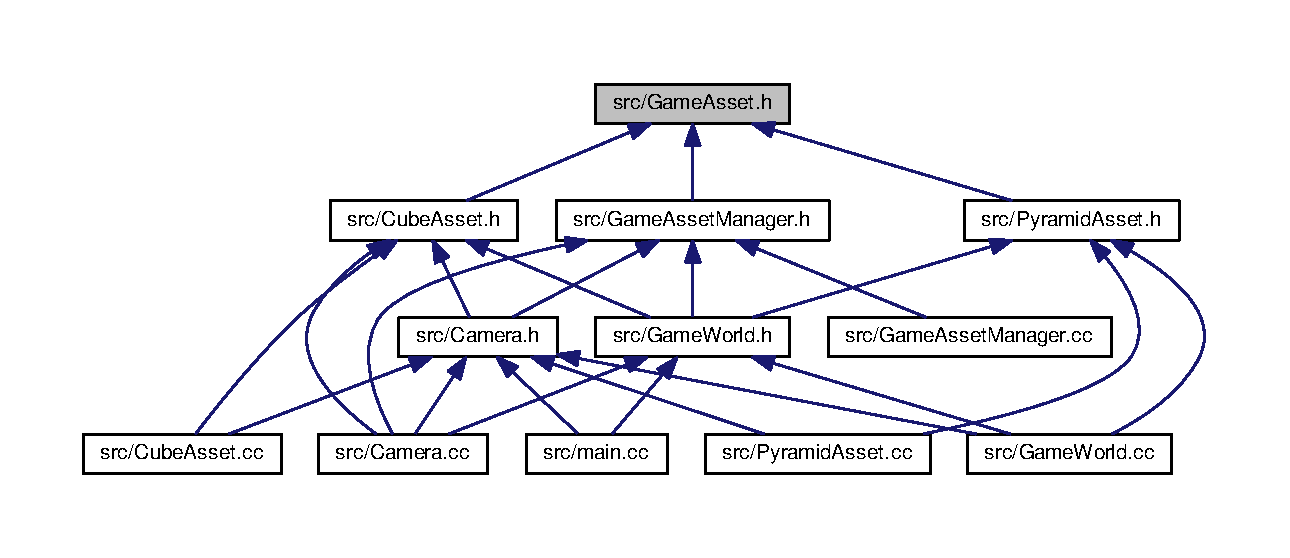
\includegraphics[width=350pt]{_game_asset_8h__dep__incl}
\end{center}
\end{figure}
\subsection*{Classes}
\begin{DoxyCompactItemize}
\item 
class \hyperlink{class_game_asset}{Game\+Asset}
\end{DoxyCompactItemize}

\hypertarget{_game_asset_manager_8cc}{}\section{src/\+Game\+Asset\+Manager.cc File Reference}
\label{_game_asset_manager_8cc}\index{src/\+Game\+Asset\+Manager.\+cc@{src/\+Game\+Asset\+Manager.\+cc}}
{\ttfamily \#include \char`\"{}Game\+Asset\+Manager.\+h\char`\"{}}\\*
Include dependency graph for Game\+Asset\+Manager.\+cc\+:
\nopagebreak
\begin{figure}[H]
\begin{center}
\leavevmode
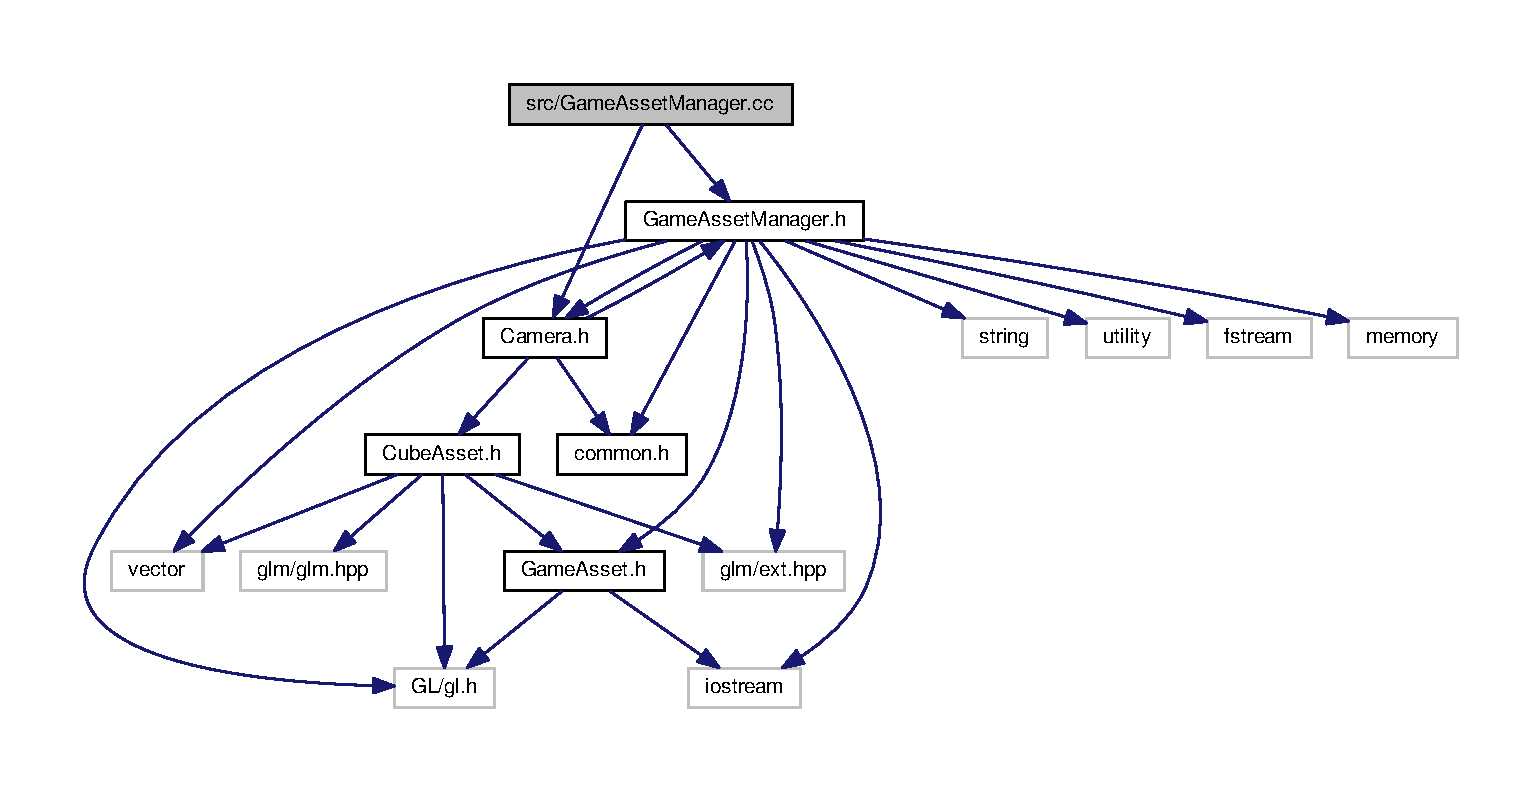
\includegraphics[width=350pt]{_game_asset_manager_8cc__incl}
\end{center}
\end{figure}
\subsection*{Variables}
\begin{DoxyCompactItemize}
\item 
class \hyperlink{class_camera}{Camera} \hyperlink{_game_asset_manager_8cc_af5a10609f4013f8e9b1ca2813ed8f526}{cam}
\end{DoxyCompactItemize}


\subsection{Variable Documentation}
\hypertarget{_game_asset_manager_8cc_af5a10609f4013f8e9b1ca2813ed8f526}{}\index{Game\+Asset\+Manager.\+cc@{Game\+Asset\+Manager.\+cc}!cam@{cam}}
\index{cam@{cam}!Game\+Asset\+Manager.\+cc@{Game\+Asset\+Manager.\+cc}}
\subsubsection[{cam}]{\setlength{\rightskip}{0pt plus 5cm}class {\bf Camera} cam}\label{_game_asset_manager_8cc_af5a10609f4013f8e9b1ca2813ed8f526}


Definition at line 3 of file Game\+Asset\+Manager.\+cc.


\hypertarget{_game_asset_manager_8h}{}\section{src/\+Game\+Asset\+Manager.h File Reference}
\label{_game_asset_manager_8h}\index{src/\+Game\+Asset\+Manager.\+h@{src/\+Game\+Asset\+Manager.\+h}}
{\ttfamily \#include $<$memory$>$}\\*
{\ttfamily \#include $<$vector$>$}\\*
{\ttfamily \#include $<$string$>$}\\*
{\ttfamily \#include $<$utility$>$}\\*
{\ttfamily \#include $<$fstream$>$}\\*
{\ttfamily \#include $<$iostream$>$}\\*
{\ttfamily \#include $<$G\+L/gl.\+h$>$}\\*
{\ttfamily \#include \char`\"{}common.\+h\char`\"{}}\\*
{\ttfamily \#include \char`\"{}Game\+Asset.\+h\char`\"{}}\\*
Include dependency graph for Game\+Asset\+Manager.\+h\+:
\nopagebreak
\begin{figure}[H]
\begin{center}
\leavevmode
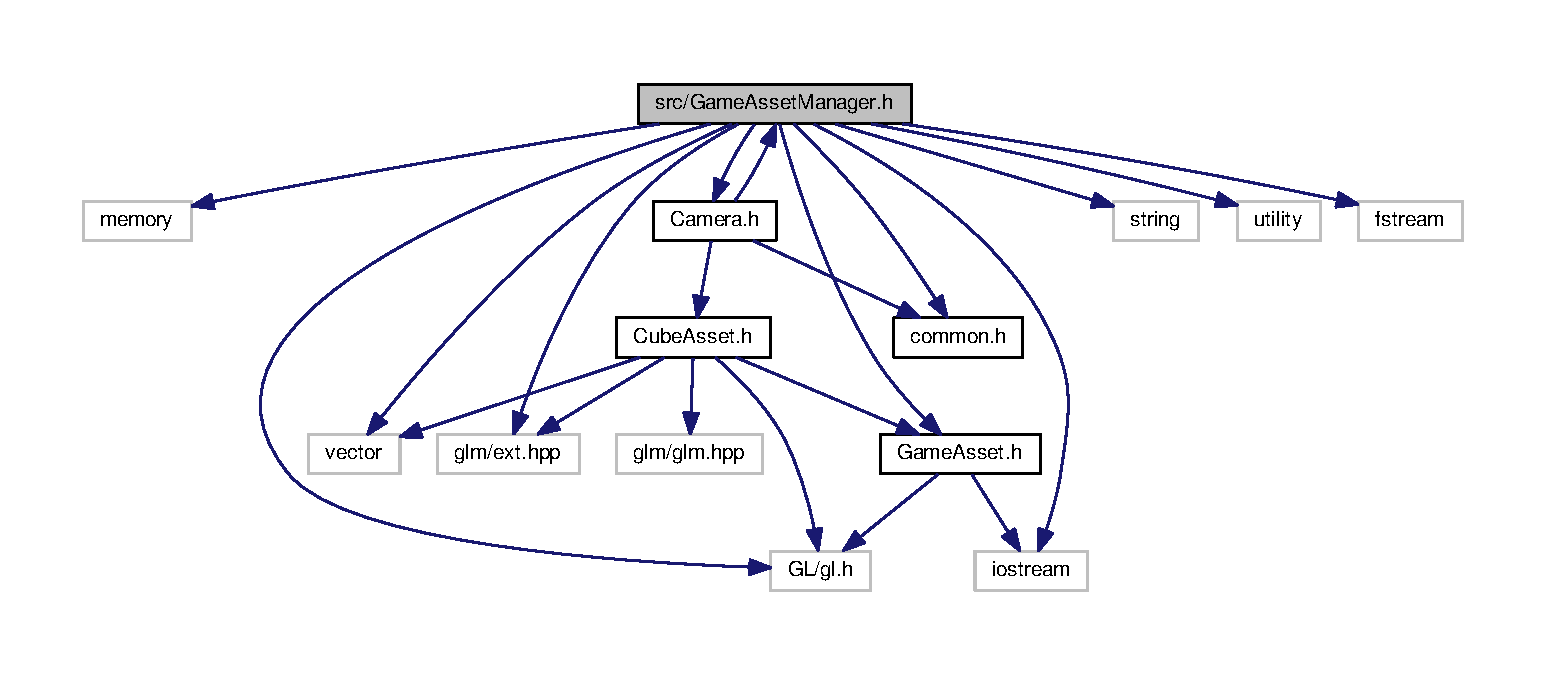
\includegraphics[width=350pt]{_game_asset_manager_8h__incl}
\end{center}
\end{figure}
This graph shows which files directly or indirectly include this file\+:
\nopagebreak
\begin{figure}[H]
\begin{center}
\leavevmode
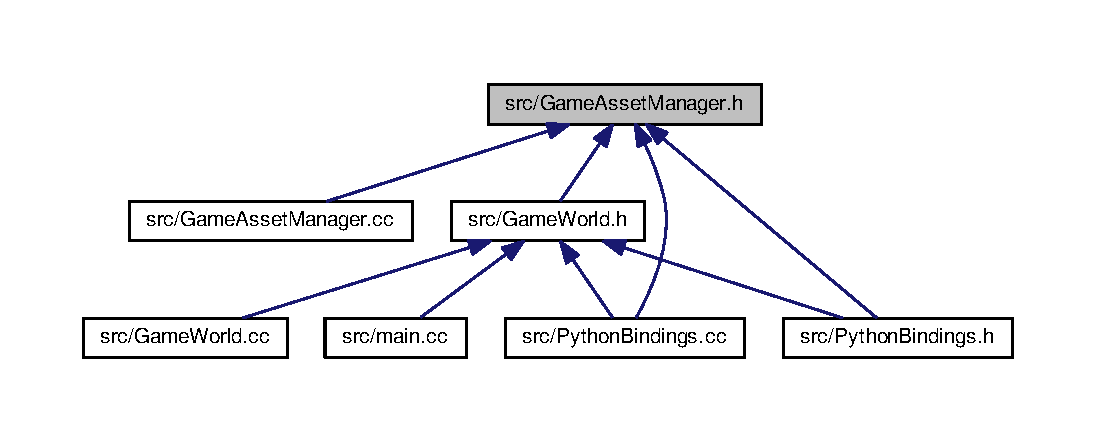
\includegraphics[width=350pt]{_game_asset_manager_8h__dep__incl}
\end{center}
\end{figure}
\subsection*{Classes}
\begin{DoxyCompactItemize}
\item 
class \hyperlink{class_game_asset_manager}{Game\+Asset\+Manager}
\end{DoxyCompactItemize}

\hypertarget{_game_world_8cc}{}\section{src/\+Game\+World.cc File Reference}
\label{_game_world_8cc}\index{src/\+Game\+World.\+cc@{src/\+Game\+World.\+cc}}
{\ttfamily \#include \char`\"{}Game\+World.\+h\char`\"{}}\\*
{\ttfamily \#include $<$Camera.\+h$>$}\\*
{\ttfamily \#include $<$Pyramid\+Asset.\+h$>$}\\*
Include dependency graph for Game\+World.\+cc\+:
\nopagebreak
\begin{figure}[H]
\begin{center}
\leavevmode
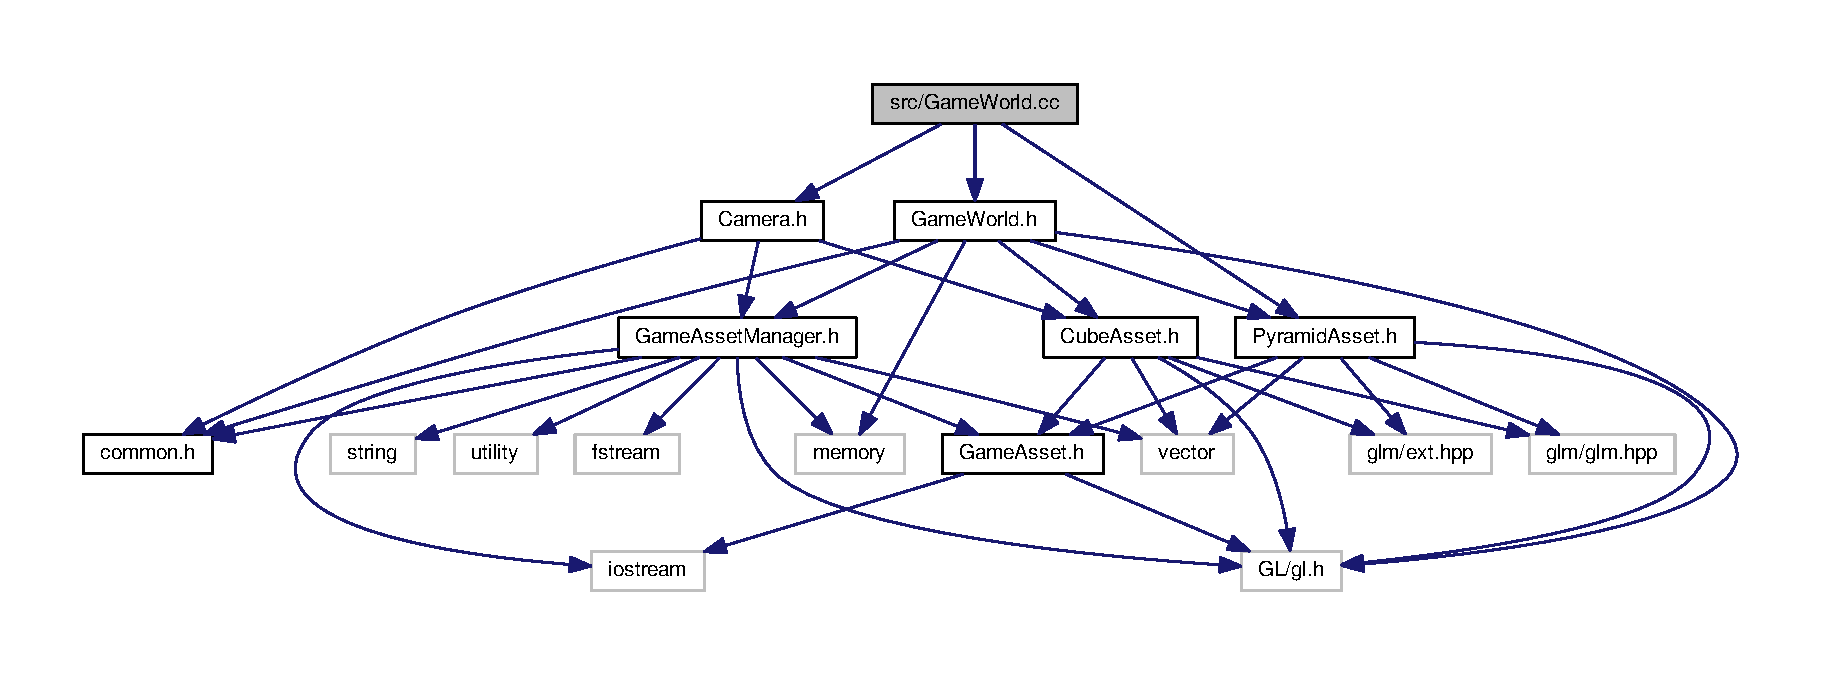
\includegraphics[width=350pt]{_game_world_8cc__incl}
\end{center}
\end{figure}

\hypertarget{_game_world_8h}{}\section{src/\+Game\+World.h File Reference}
\label{_game_world_8h}\index{src/\+Game\+World.\+h@{src/\+Game\+World.\+h}}
{\ttfamily \#include $<$memory$>$}\\*
{\ttfamily \#include $<$G\+L/gl.\+h$>$}\\*
{\ttfamily \#include \char`\"{}common.\+h\char`\"{}}\\*
{\ttfamily \#include \char`\"{}Game\+Asset\+Manager.\+h\char`\"{}}\\*
{\ttfamily \#include \char`\"{}Cube\+Asset.\+h\char`\"{}}\\*
{\ttfamily \#include \char`\"{}Pyramid\+Asset.\+h\char`\"{}}\\*
{\ttfamily \#include \char`\"{}Camera.\+h\char`\"{}}\\*
Include dependency graph for Game\+World.\+h\+:
\nopagebreak
\begin{figure}[H]
\begin{center}
\leavevmode
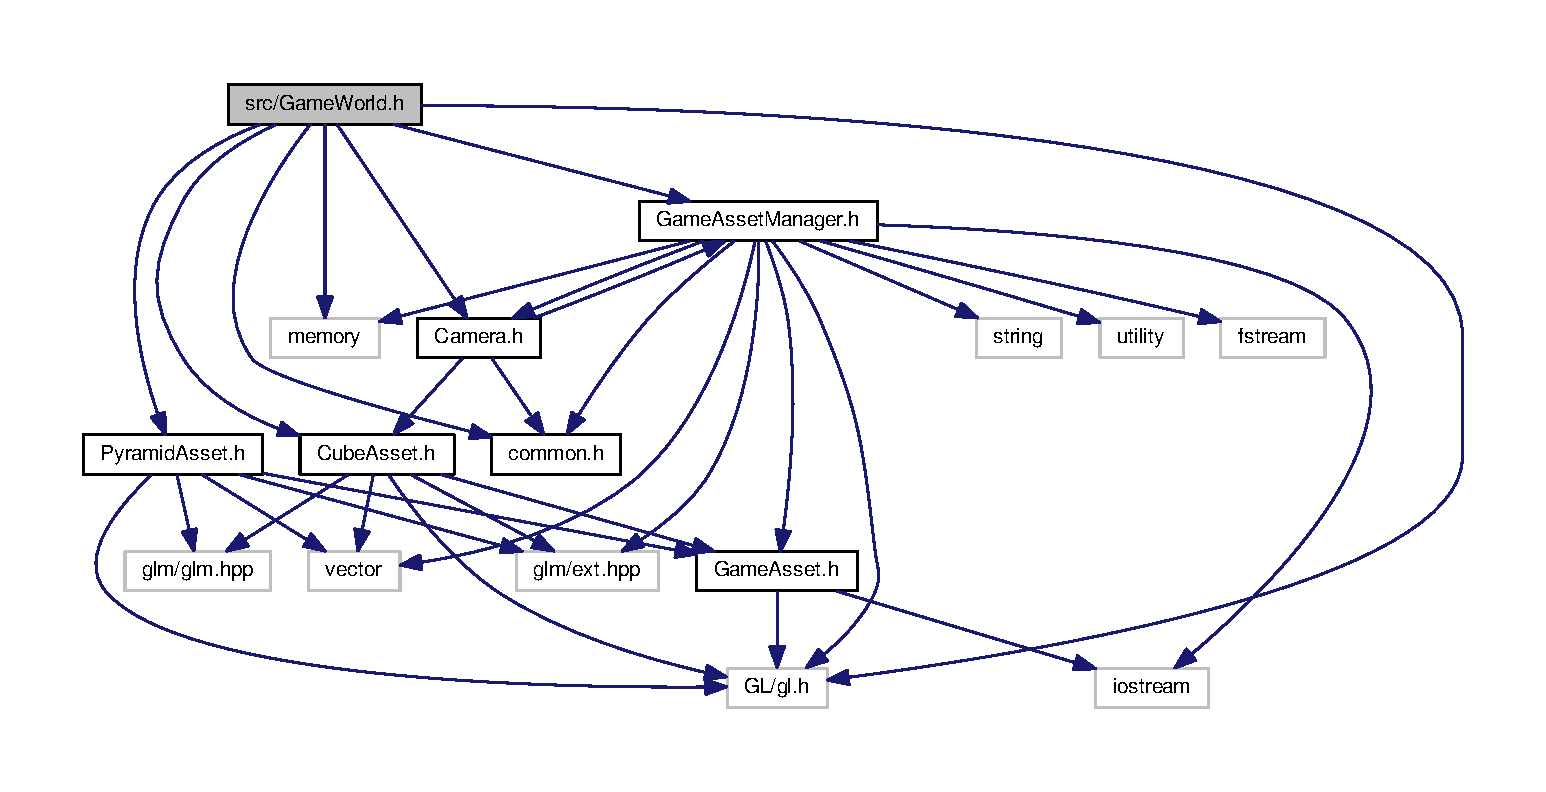
\includegraphics[width=350pt]{_game_world_8h__incl}
\end{center}
\end{figure}
This graph shows which files directly or indirectly include this file\+:
\nopagebreak
\begin{figure}[H]
\begin{center}
\leavevmode
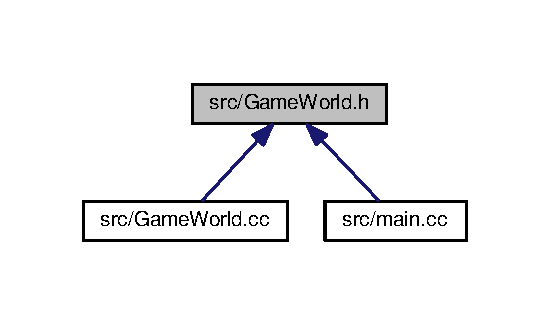
\includegraphics[width=264pt]{_game_world_8h__dep__incl}
\end{center}
\end{figure}
\subsection*{Classes}
\begin{DoxyCompactItemize}
\item 
class \hyperlink{class_game_world}{Game\+World}
\end{DoxyCompactItemize}

\hypertarget{main_8cc}{}\section{src/main.cc File Reference}
\label{main_8cc}\index{src/main.\+cc@{src/main.\+cc}}
{\ttfamily \#include $<$G\+L/glew.\+h$>$}\\*
{\ttfamily \#include $<$G\+L/gl.\+h$>$}\\*
{\ttfamily \#include $<$S\+D\+L2/\+S\+D\+L.\+h$>$}\\*
{\ttfamily \#include $<$iostream$>$}\\*
{\ttfamily \#include $<$memory$>$}\\*
{\ttfamily \#include $<$boost/program\+\_\+options.\+hpp$>$}\\*
{\ttfamily \#include \char`\"{}common.\+h\char`\"{}}\\*
{\ttfamily \#include \char`\"{}Game\+World.\+h\char`\"{}}\\*
{\ttfamily \#include \char`\"{}Camera.\+h\char`\"{}}\\*
Include dependency graph for main.\+cc\+:\nopagebreak
\begin{figure}[H]
\begin{center}
\leavevmode
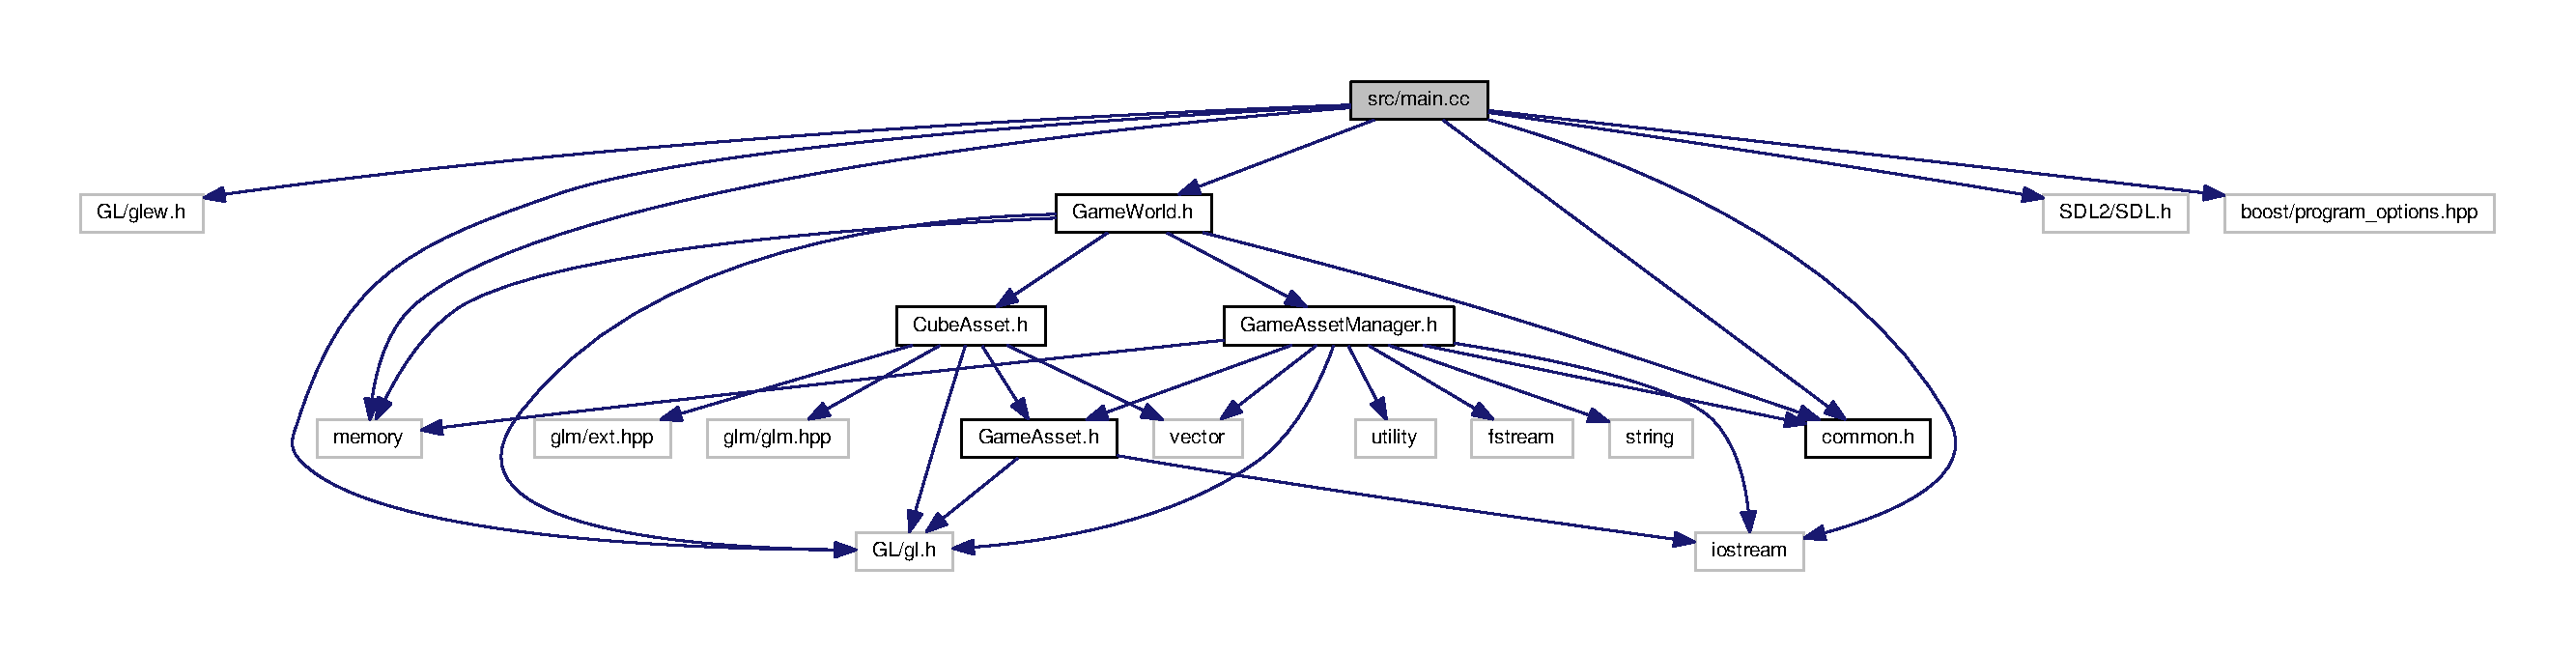
\includegraphics[width=350pt]{main_8cc__incl}
\end{center}
\end{figure}
\subsection*{Classes}
\begin{DoxyCompactItemize}
\item 
struct \hyperlink{struct_s_d_l_window_deleter}{S\+D\+L\+Window\+Deleter}
\end{DoxyCompactItemize}
\subsection*{Macros}
\begin{DoxyCompactItemize}
\item 
\#define \hyperlink{main_8cc_abcde84ea0ef5f934384e4620f092c85a}{G\+L\+E\+W\+\_\+\+S\+T\+A\+T\+I\+C}
\item 
\#define \hyperlink{main_8cc_a6ff0ea1b288e03115f981ba31f96fade}{R\+U\+N\+\_\+\+G\+R\+A\+P\+H\+I\+C\+S\+\_\+\+D\+I\+S\+P\+L\+A\+Y}~0x00;
\end{DoxyCompactItemize}
\subsection*{Functions}
\begin{DoxyCompactItemize}
\item 
Uint32 \hyperlink{main_8cc_a70eaa727262f633037c3f4b7d3ff24c2}{tick} (Uint32 interval, void $\ast$param)
\item 
void \hyperlink{main_8cc_afd34c13fc4f409851ffc0989c13dd287}{Draw} (const std\+::shared\+\_\+ptr$<$ S\+D\+L\+\_\+\+Window $>$ window, const std\+::shared\+\_\+ptr$<$ \hyperlink{class_game_world}{Game\+World} $>$ game\+\_\+world)
\item 
std\+::shared\+\_\+ptr$<$ S\+D\+L\+\_\+\+Window $>$ \hyperlink{main_8cc_acab7ade71cf38099442ca5df2495223d}{Init\+World} ()
\item 
\hyperlink{common_8h_add86e7c88dd109abea3f708b422f31f0}{Application\+Mode} \hyperlink{main_8cc_aba227fab3b52f0ce7c5b89d75b88dcdc}{Parse\+Options} (int argc, char $\ast$$\ast$argv)
\item 
int \hyperlink{main_8cc_a3c04138a5bfe5d72780bb7e82a18e627}{main} (int argc, char $\ast$$\ast$argv)
\end{DoxyCompactItemize}


\subsection{Macro Definition Documentation}
\hypertarget{main_8cc_abcde84ea0ef5f934384e4620f092c85a}{}\index{main.\+cc@{main.\+cc}!G\+L\+E\+W\+\_\+\+S\+T\+A\+T\+I\+C@{G\+L\+E\+W\+\_\+\+S\+T\+A\+T\+I\+C}}
\index{G\+L\+E\+W\+\_\+\+S\+T\+A\+T\+I\+C@{G\+L\+E\+W\+\_\+\+S\+T\+A\+T\+I\+C}!main.\+cc@{main.\+cc}}
\subsubsection[{G\+L\+E\+W\+\_\+\+S\+T\+A\+T\+I\+C}]{\setlength{\rightskip}{0pt plus 5cm}\#define G\+L\+E\+W\+\_\+\+S\+T\+A\+T\+I\+C}\label{main_8cc_abcde84ea0ef5f934384e4620f092c85a}


Definition at line 1 of file main.\+cc.

\hypertarget{main_8cc_a6ff0ea1b288e03115f981ba31f96fade}{}\index{main.\+cc@{main.\+cc}!R\+U\+N\+\_\+\+G\+R\+A\+P\+H\+I\+C\+S\+\_\+\+D\+I\+S\+P\+L\+A\+Y@{R\+U\+N\+\_\+\+G\+R\+A\+P\+H\+I\+C\+S\+\_\+\+D\+I\+S\+P\+L\+A\+Y}}
\index{R\+U\+N\+\_\+\+G\+R\+A\+P\+H\+I\+C\+S\+\_\+\+D\+I\+S\+P\+L\+A\+Y@{R\+U\+N\+\_\+\+G\+R\+A\+P\+H\+I\+C\+S\+\_\+\+D\+I\+S\+P\+L\+A\+Y}!main.\+cc@{main.\+cc}}
\subsubsection[{R\+U\+N\+\_\+\+G\+R\+A\+P\+H\+I\+C\+S\+\_\+\+D\+I\+S\+P\+L\+A\+Y}]{\setlength{\rightskip}{0pt plus 5cm}\#define R\+U\+N\+\_\+\+G\+R\+A\+P\+H\+I\+C\+S\+\_\+\+D\+I\+S\+P\+L\+A\+Y~0x00;}\label{main_8cc_a6ff0ea1b288e03115f981ba31f96fade}


Definition at line 10 of file main.\+cc.



\subsection{Function Documentation}
\hypertarget{main_8cc_afd34c13fc4f409851ffc0989c13dd287}{}\index{main.\+cc@{main.\+cc}!Draw@{Draw}}
\index{Draw@{Draw}!main.\+cc@{main.\+cc}}
\subsubsection[{Draw(const std\+::shared\+\_\+ptr$<$ S\+D\+L\+\_\+\+Window $>$ window, const std\+::shared\+\_\+ptr$<$ Game\+World $>$ game\+\_\+world)}]{\setlength{\rightskip}{0pt plus 5cm}void Draw (
\begin{DoxyParamCaption}
\item[{const std\+::shared\+\_\+ptr$<$ S\+D\+L\+\_\+\+Window $>$}]{window, }
\item[{const std\+::shared\+\_\+ptr$<$ {\bf Game\+World} $>$}]{game\+\_\+world}
\end{DoxyParamCaption}
)}\label{main_8cc_afd34c13fc4f409851ffc0989c13dd287}


Definition at line 38 of file main.\+cc.

\hypertarget{main_8cc_acab7ade71cf38099442ca5df2495223d}{}\index{main.\+cc@{main.\+cc}!Init\+World@{Init\+World}}
\index{Init\+World@{Init\+World}!main.\+cc@{main.\+cc}}
\subsubsection[{Init\+World()}]{\setlength{\rightskip}{0pt plus 5cm}std\+::shared\+\_\+ptr$<$S\+D\+L\+\_\+\+Window$>$ Init\+World (
\begin{DoxyParamCaption}
{}
\end{DoxyParamCaption}
)}\label{main_8cc_acab7ade71cf38099442ca5df2495223d}


Definition at line 50 of file main.\+cc.

\hypertarget{main_8cc_a3c04138a5bfe5d72780bb7e82a18e627}{}\index{main.\+cc@{main.\+cc}!main@{main}}
\index{main@{main}!main.\+cc@{main.\+cc}}
\subsubsection[{main(int argc, char $\ast$$\ast$argv)}]{\setlength{\rightskip}{0pt plus 5cm}int main (
\begin{DoxyParamCaption}
\item[{int}]{argc, }
\item[{char $\ast$$\ast$}]{argv}
\end{DoxyParamCaption}
)}\label{main_8cc_a3c04138a5bfe5d72780bb7e82a18e627}


Definition at line 143 of file main.\+cc.



Here is the call graph for this function\+:\nopagebreak
\begin{figure}[H]
\begin{center}
\leavevmode
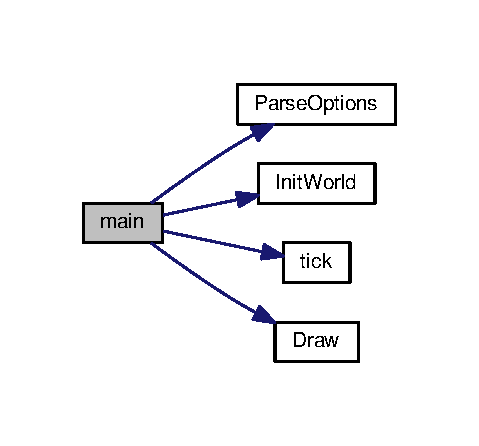
\includegraphics[width=230pt]{main_8cc_a3c04138a5bfe5d72780bb7e82a18e627_cgraph}
\end{center}
\end{figure}


\hypertarget{main_8cc_aba227fab3b52f0ce7c5b89d75b88dcdc}{}\index{main.\+cc@{main.\+cc}!Parse\+Options@{Parse\+Options}}
\index{Parse\+Options@{Parse\+Options}!main.\+cc@{main.\+cc}}
\subsubsection[{Parse\+Options(int argc, char $\ast$$\ast$argv)}]{\setlength{\rightskip}{0pt plus 5cm}{\bf Application\+Mode} Parse\+Options (
\begin{DoxyParamCaption}
\item[{int}]{argc, }
\item[{char $\ast$$\ast$}]{argv}
\end{DoxyParamCaption}
)}\label{main_8cc_aba227fab3b52f0ce7c5b89d75b88dcdc}


Definition at line 111 of file main.\+cc.

\hypertarget{main_8cc_a70eaa727262f633037c3f4b7d3ff24c2}{}\index{main.\+cc@{main.\+cc}!tick@{tick}}
\index{tick@{tick}!main.\+cc@{main.\+cc}}
\subsubsection[{tick(\+Uint32 interval, void $\ast$param)}]{\setlength{\rightskip}{0pt plus 5cm}Uint32 tick (
\begin{DoxyParamCaption}
\item[{Uint32}]{interval, }
\item[{void $\ast$}]{param}
\end{DoxyParamCaption}
)}\label{main_8cc_a70eaa727262f633037c3f4b7d3ff24c2}


Definition at line 22 of file main.\+cc.


%--- End generated contents ---

% Index
\backmatter
\newpage
\phantomsection
\clearemptydoublepage
\addcontentsline{toc}{chapter}{Index}
\printindex

\end{document}
